\chapter{Resultados}
\label{capitulo6}
\lhead{Capítulo 6. \emph{Resultados}}

En el capítulo anterior, se detalló la implementación de la solución propuesta para abordar el problema de evasión de obstáculos en QUAVs, centrándose en la metodología, la plataforma de implementación, la justificación del algoritmo seleccionado y la descripción del funcionamiento de los componentes principales. Este capítulo se adentra ahora en la evaluación y presentación de los resultados obtenidos, proporcionando una perspectiva crítica sobre el rendimiento de la solución propuesta.

En la sección \ref{sec:results-finetune} se examinan los resultados del ajuste fino de la política estudiante, destacando los desafíos asociados al sobre-ajuste de los datos de entrenamiento y a la generación de la base de datos. Además, se exploran las consecuencias derivadas de estos problemas al evaluar la política de evasión de obstáculos.

La sección \ref{sec:results-flights} examina los resultados de la política de evasión de obstáculos, dividida en dos subsecciones clave: la subsección \ref{sec:results-AirSim}, que presenta los resultados de vuelos en simulación, y la subsección \ref{sec:results-SOTEN}, centrada en vuelos sobre la plataforma física de implementación, SOTEN. Estos resultados ofrecen una perspectiva del rendimiento de la solución en configuraciones simples de obstáculos, donde la política de evasión se muestra estable. Además, se evalúan otras configuraciones de obstáculos en donde política no logra completar su función de manera satisfactoria, y se identifica la relación entre este resultado y los desafíos asociados al ajuste fino de la política estudiante.

El análisis detallado de estos resultados proporciona una evaluación crítica de la efectividad de la solución propuesta, sirviendo como base para la discusión en el siguiente capítulo. Aquí, se extraerán conclusiones significativas y se identificarán posibles direcciones para mejorar el rendimiento en futuras investigaciones en el campo de evasión de obstáculos en QUAVs.

\section{Resultados del ajuste fino de la política estudiante}

\label{sec:results-finetune}

Como se menciono en el capitulo anterior, el objetivo del ajuste fino de la política estudiante, es ajustar los pesos provistos por \cite{Loquercio2021} para que la red neuronal genere trayectorias con \jim{v_{des} = 1} m/s; idealmente, manteniendo un nivel de generalización comparable a la de los pesos provistos por \cite{Loquercio2021}. Recordando que la función de pérdida de la red neuronal de \cite{Loquercio2021} tiene dos componen es: un componente espacial que cuantifica que tan cerca se encuentran las trayectorias predichas a las generadas por el experto, y un componente de estimación que cuantifica que tan correctamente se hace la estimación del costo de ejecución \jim{c_k}; las figuras \ref{fig:loss-space-all} y \ref{fig:loss-estim-all} muestran el valor del componente espacial y de estimación en función de las épocas, tanto para el conjunto de entrenamiento como para el de validación.

\begin{figure}[H]
    \centering
    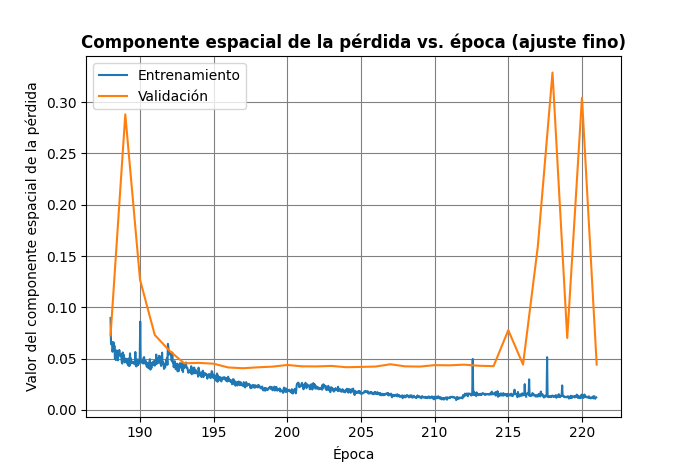
\includegraphics[scale=0.65]{partes/ImgJoao/loss-space-all.png}
    \caption[Componente espacial de la pérdida vs. época (ajuste fino).]{Componente espacial de la pérdida vs. época (ajuste fino). Se observa claramente la divergencia de la perdida sobre el conjunto de validación a partir de la época 215.}
    \label{fig:loss-space-all}
\end{figure}

\begin{figure}[H]
    \centering
    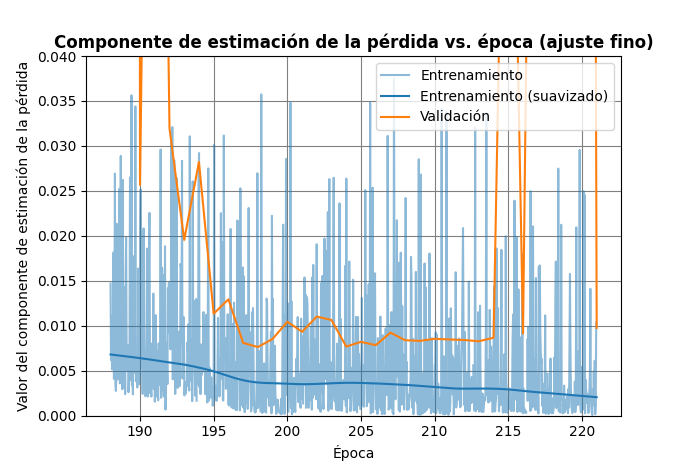
\includegraphics[scale=0.65]{partes/ImgJoao/loss-estim-all.png}
    \caption[Componente de estimación de la pérdida vs. época (ajuste fino).]{Componente de estimación de la pérdida vs. época (ajuste fino). Se observa claramente la divergencia de la pérdida sobre el conjunto de validación a partir de la época 215.}
    \label{fig:loss-estim-all}
\end{figure}

Las figuras \ref{fig:loss-space-all} y \ref{fig:loss-estim-all} reflejan la divergencia del valor de la pérdida sobre el conjunto de validación a partir de la época 215. Para contrarrestar este efecto, se decidió utilizar un punto de control temprano antes de la divergencia, efectivamente deteniendo el entrenamiento de forma temprana. El punto de control mas cercano anterior a la época 215 fue el punto de control de la época 213. Al regresar a dicho punto de control se elimino la divergencia del valor de pérdida de validación. Las figuras \ref{fig:loss-space-stopped} y \ref{fig:loss-estim-stopped} muestran el valor del componente espacial y de estimación en función de las épocas luego de detener tempranamente el entrenamiento, tanto para el conjunto de entrenamiento como para el de validación. Eliminando la divergencia de la pérdida de validación, se puede proceder a a evaluar este modelo contra el modelo original provisto por \cite{Loquercio2021}. Como las métricas de \cite{Loquercio2021} evalúan el sistema completo, la única métrica que se puede utilizar para comparar modelos es el valor de la función de pérdida a lo largo de un conjunto de datos. Para que esta comparación sea efectiva, lo importante es seleccionar conjuntos de datos representativos de la comparación deseada; precisamente eso es lo que se realizó y se describe a continuación.

\begin{figure}[H]
    \centering
    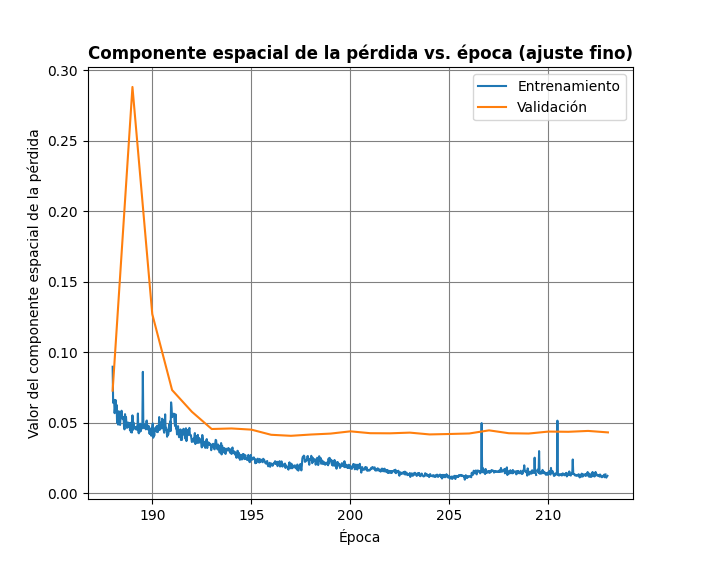
\includegraphics[scale=0.65]{partes/ImgJoao/loss-space-stopped.png}
    \caption[Componente espacial de la pérdida vs. época (ajuste fino) luego de detener el entrenamiento tempranamente.]{Componente espacial de la pérdida vs. época (ajuste fino) luego de detener el entrenamiento tempranamente. No se observa divergencia en el valor de la pérdida sobre el conjunto de validación.}
    \label{fig:loss-space-stopped}
\end{figure}

\begin{figure}[H]
    \centering
    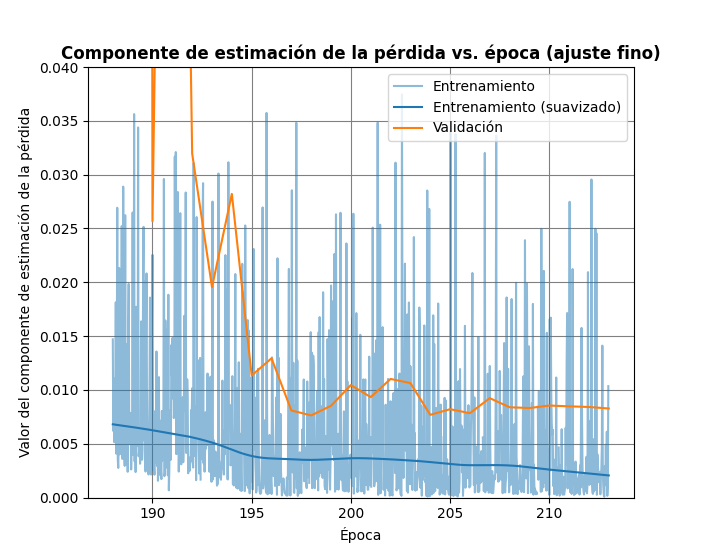
\includegraphics[scale=0.65]{partes/ImgJoao/loss-estim-stopped.png}
    \caption[Componente de estimación de la pérdida vs. época (ajuste fino) luego de detener el entrenamiento tempranamente.]{Componente de estimación de la pérdida vs. época (ajuste fino) luego de detener el entrenamiento tempranamente. No se observa divergencia en el valor de la pérdida sobre el conjunto de validación.}
    \label{fig:loss-estim-stopped}
\end{figure}

Los modelos a comparar son el modelo original, que destaca en la capacidad de predecir trayectorias sin colisión con \jim{v_{des} = 7} m/s; y el modelo ajustado en este trabajo para predecir trayectorias sin colisión con \jim{v_{des} = 1} m/s. Para ello, se seleccionaron dos conjuntos de datos, el conjunto de datos de validación con trayectorias con \jim{v_{des} = 7} m/s (obtenido del repositorio de \cite{Loquercio2021}) y el conjunto de datos de validación con las trayectorias con \jim{v_{des} = 1} m/s (el generado en el presente trabajo). La diferencia en los valores de pérdida entre esos modelos y conjuntos de datos, dan una idea del rendimiento relativo de cada uno de los modelos dentro de los escenarios presenciados en el conjunto de datos. Las figura \ref{fig:loss-space-bars} y \ref{fig:loss-estim-bars} muestran una visualización de esta comparación.

\begin{figure}[H]
    \centering
    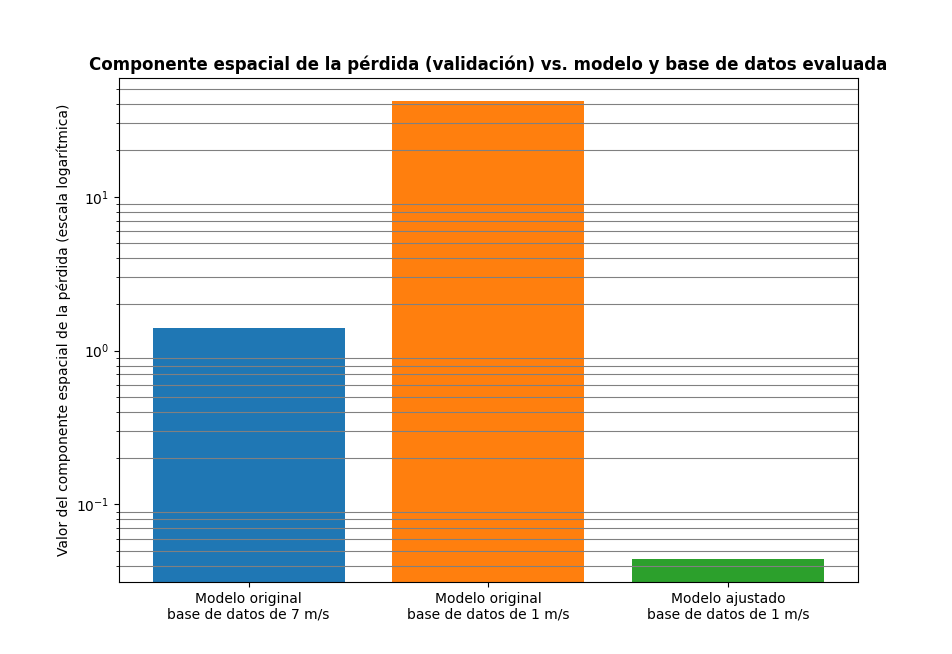
\includegraphics[scale=0.6]{partes/ImgJoao/loss-space-bars.png}
    \caption[Comparación de los valores del componente de pérdida espacial entre modelo original y modelo ajustado.]{Comparación de los valores de pérdida entre modelo original y modelo ajustado.}
    \label{fig:loss-space-bars}
\end{figure}

\begin{figure}[H]
    \centering
    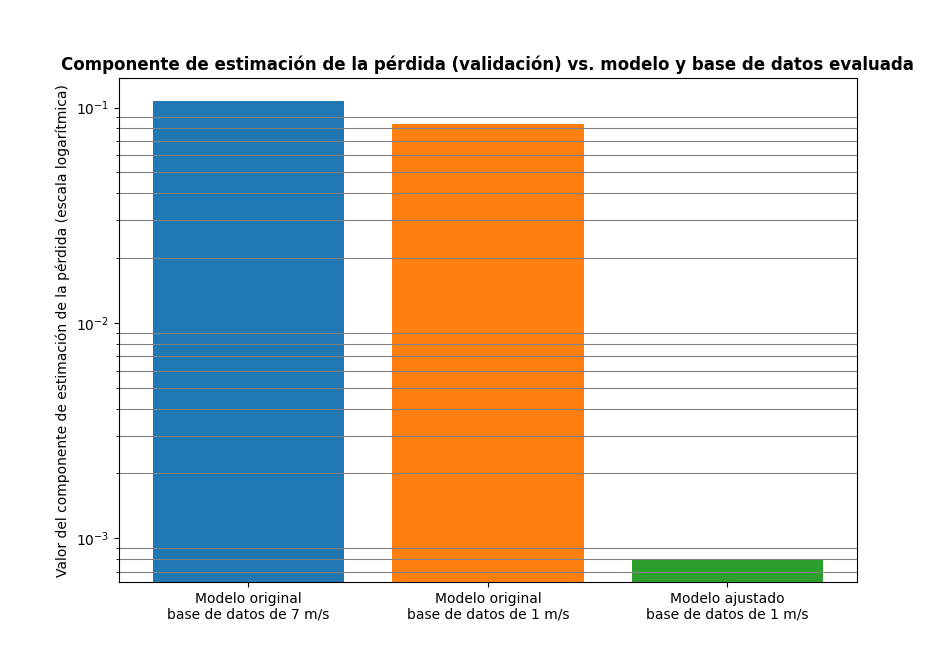
\includegraphics[scale=0.6]{partes/ImgJoao/loss-estim-bars.png}
    \caption[Comparación de los valores del componente de pérdida de estimación entre modelo original y modelo ajustado.]{Comparación de los valores del componente de pérdida de estimación entre modelo original y modelo ajustado.}
    \label{fig:loss-estim-bars}
\end{figure}

De esta comparación podemos realizar algunas observaciones relevantes. Primero, el modelo original tiene dificultades en generar trayectorias con las características espaciales de las trayectorias con \jim{v_{des} = 1} m/s, esto tiene sentido pues la diferencia espacial entre moverse a 7 m/s y 1 m/s es bastante alta; esto simplemente confirma la dependencia entre \jim{v_{des}} del experto y el despeñó de la política estudiante a distintas velocidades, tal como se afirma en \cite{Loquercio2021}. Por otro lado, el modelo original logra generalizar la tarea de estimar el costo de ejecución de una trayectoria, los valores del componente de estimación de la pérdida están en el mismo orden tanto para \jim{v_{des} = 7} m/s como para \jim{v_{des} = 1} m/s. 

Segundo, y mas relevante para este trabajo, los valores de pérdida del modelo ajustado sobre el conjunto con \jim{v_{des} = 1} m/s están dos ordenes de magnitud por debajo de los valores del modelo original sobre el conjunto con \jim{v_{des} = 7} m/s; esto puede indicar la presencia de sobre-ajuste (pérdida de capacidad de generalización), sin embargo, este sobre-ajuste no existe al nivel de conjuntos de entrenamiento y de validación, pero al nivel de los conjuntos de datos generados por el experto con distintos valores de \jim{v_{des}}. Para confirmar esta linea de pensamiento, se procede a visualizar una muestra de las trayectorias generadas con \jim{v_{des} = 1} m/s y compararlas con una muestra de las trayectorias generadas con \jim{v_{des} = 7} m/s. Si ambos conjuntos de datos tienen niveles equivalente de generalización, se debería observar en cada muestra una representación amplia de distintas trayectorias. Si alguna de las dos muestras tiene preferencia por un caso particular de trayectorias con respecto a la otra muestra, entonces esa base de datos tiene menos capacidad de generalización relativamente. De cada base de datos se seleccionaron 3 vuelos aleatoriamente, las figuras \ref{fig:7ms-sample} y \ref{fig:1ms-sample} visualizan las muestras seleccionadas. Cada muestra se visualiza como una vista ``de arriba hacia abajo'' de la nube de puntos del entorno junto con las trayectorias generadas durante el vuelo; el color de las trayectorias interpola entre azul y rojo, mientras mas rojo, mas costo de ejecución tiene la trayectoria. Este experimento se repitió 10 veces con resultados similares, para facilitar la visualización de los resultados, solo se muestra un solo experimento.

\begin{figure}[H]
    \centering
    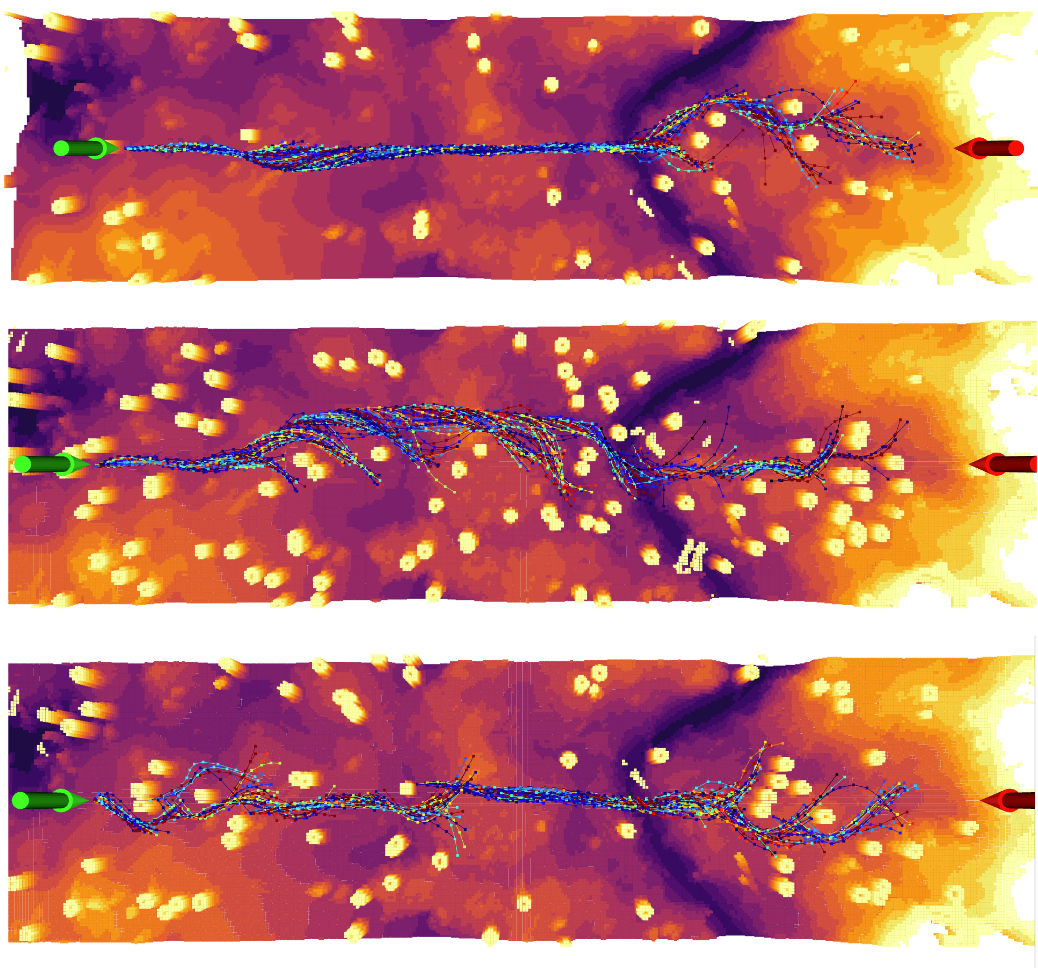
\includegraphics[scale=0.4]{partes/ImgJoao/7ms-sample.png}
    \caption[Visualización de tres vuelos de la base de datos con \jim{v_{des} = 7} m/s.]{Visualización de tres vuelos de la base de datos con \jim{v_{des} = 7} m/s.}
    \label{fig:7ms-sample}
\end{figure}

\begin{figure}[H]
    \centering
    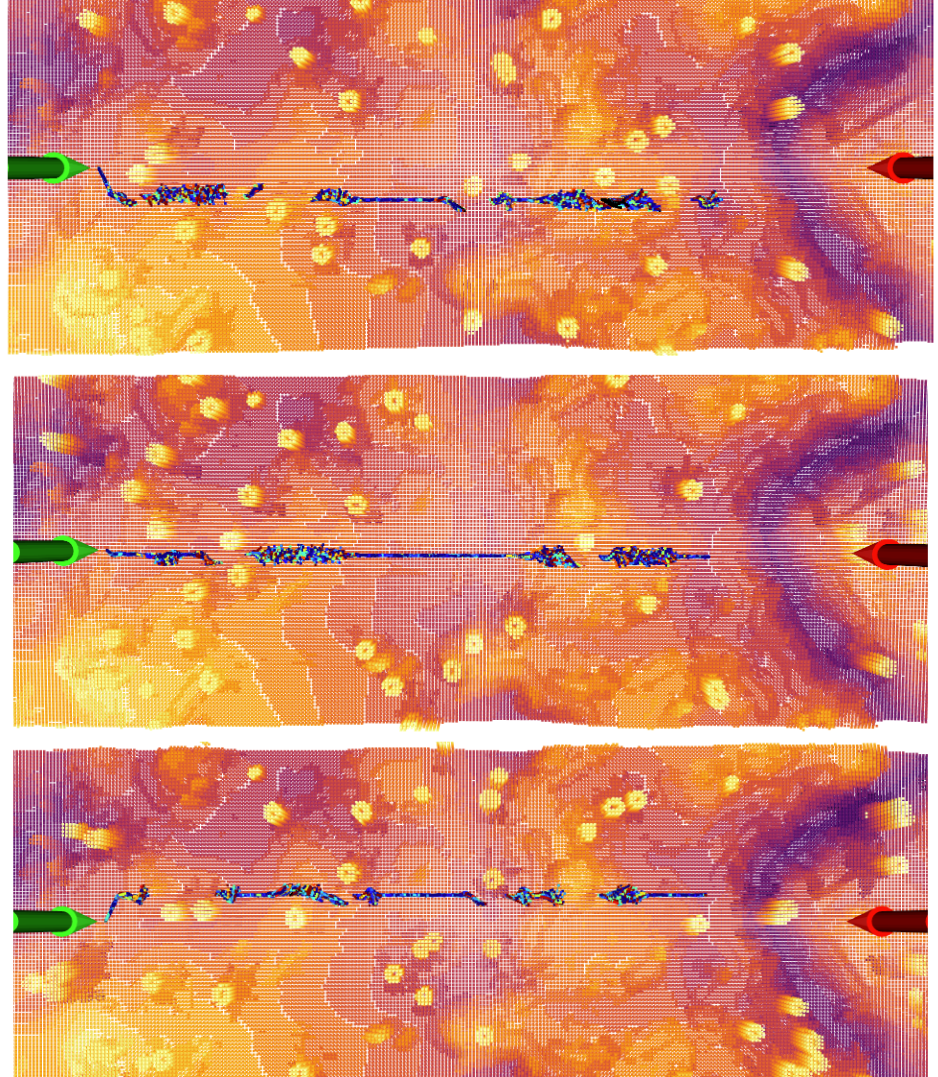
\includegraphics[scale=0.4]{partes/ImgJoao/1ms-sample.png}
    \caption[Visualización de tres vuelos de la base de datos con \jim{v_{des} = 1} m/s.]{Visualización de tres vuelos de la base de datos con \jim{v_{des} = 1} m/s.}
    \label{fig:1ms-sample}
\end{figure}

A simple vista se observa una clara diferencia, en la base de datos con \jim{v_{des} = 1} m/s, los obstáculos solo se esquivan por uno solo de los flancos del obstáculo, mientras en la base de datos con \jim{v_{des} = 7} m/s se exploran ambos flancos como posibilidades de esquivar el ósculo. Esto implícitamente muestra que la base de datos con \jim{v_{des} = 1} m/s tiene menos capacidad de generalización que la base de datos con \jim{v_{des} = 7} m/s simplemente porque tiene menos opciones en promedio para esquivar un mismo obstáculo. En otras palabras, existe un desbalance de las modas de la distribución \jim{P}\footnote{La distribución \jim{P} se describe en la ecuación \ref{eq:aoa-expert-P}} en la base de datos con \jim{v_{des} = 1} m/s que no existe significativamente en en la base de datos con \jim{v_{des} = 7} m/s. Este desbalance hace que el proceso de refinamiento fino implícitamente produzca un efecto sobre-ajuste con respecto a rendimiento de la política publicada por \cite{Loquercio2021}, el modelo se ajusta demasiado a los ejemplos de la base datos con \jim{v_{des} = 1} m/s, potencialmente reduciendo significativamente su capacidad multi-modal para producir trayectorias libre de colisión.

Un posible origen de este problema, es que la poca longitud de las trayectorias generadas para \jim{v_{des} = 1} m/s no permite que el experto genere trayectorias que consideren todas las modas de la distribución \jim{P} con un valor de costo bajo, cuando el experto selecciona las mejores 3 trayectorias, estas trayectorias se descartan produciendo el desbalance. Otra posible razón puede ser que el planificador de trayectorias globales que genera \jim{\tau_{ref}} no permita la exploración de dichas trayectorias, principalmente por planificar trayectorias triviales en donde se navegue mayoritariamente sin encontrar obstáculos. 

Una posible solución para este problema es modificar el entorno de simulación para que la configuración de los obstáculos permita que el experto considere las modas de \jim{P} con alto valor de costo, por ejemplo, incrementando la densidad de los obstáculos y reduciendo sus dimensiones. Otra posible solución es modificar los parámetros del planificador de trayectorias globales de forma que la ejecución de \jim{\tau_{ref}} fomente la exploración de obstáculos en donde se generen muestras que representen el carácter multi-modal de \jim{P}, por ejemplo, intencionalmente dirigiéndose hacia la cercanía de grupos de obstáculos. Alternativamente se pueden ejecutar las predicciones de la red en lugar de seguir una \jim{\tau_{ref}} planificada globalmente, y en su lugar utilizar una \jim{\tau_{ref}} que simplemente sea el camino en linea recta desde el punto de despegue hasta la meta; esto potencialmente va a incrementar la exploración de obstáculos en donde se generen muestras que representen múltiples moda de \jim{P}.

Dicho esto, por limitaciones del tiempo de desarrollo de este trabajo y recomendaciones por parte del equipo de ACSL; en este trabajo no se soluciona el problema descrito anteriormente. Esto significa que la política estudiante utilizada en este trabajo sufre las consecuencias del sobre-ajuste ocasionado por el desbalance de modas en la base de datos con \jim{v_{des} = 1} m/s, esto puede ocasionar que la política de evasión de obstáculos tenga una preferencia fuerte en esquivar obstáculos de una forma en particular. En las siguientes secciones observaremos que efectivamente, la política de evasión de obstáculos tiene una fuerte preferencia a esquivar obstáculos por el flanco izquierdo, y observaremos como este comportamiento hace que la ejecución en entornos no triviales termine en potenciales colisiones.

\section{Resultados de la política de evasión de obstáculos}

\label{sec:results-flights}

\subsection{Vuelos en entorno simulación}

\label{sec:results-AirSim}

En esta sección se describen las configuraciones de los vuelos realizados en el entorno de simulación AirSim \cite{shah2018airsim}, así como también sus resultados y comportamientos observados. La primera configuración de obstáculos utilizada es una configuración simple con un solo obstáculo en la linea directa de visión del QUAV, un diagrama de la configuración se muestra en la figura \ref{fig:config-1-single}. En el diagrama se muestran dos vistas, la frontal (plano \jim{yz}) a partir desde el punto de despegue y la vista de arriba hacia abajo (plano \jim{xy}).

\begin{figure}[H]
    \centering
    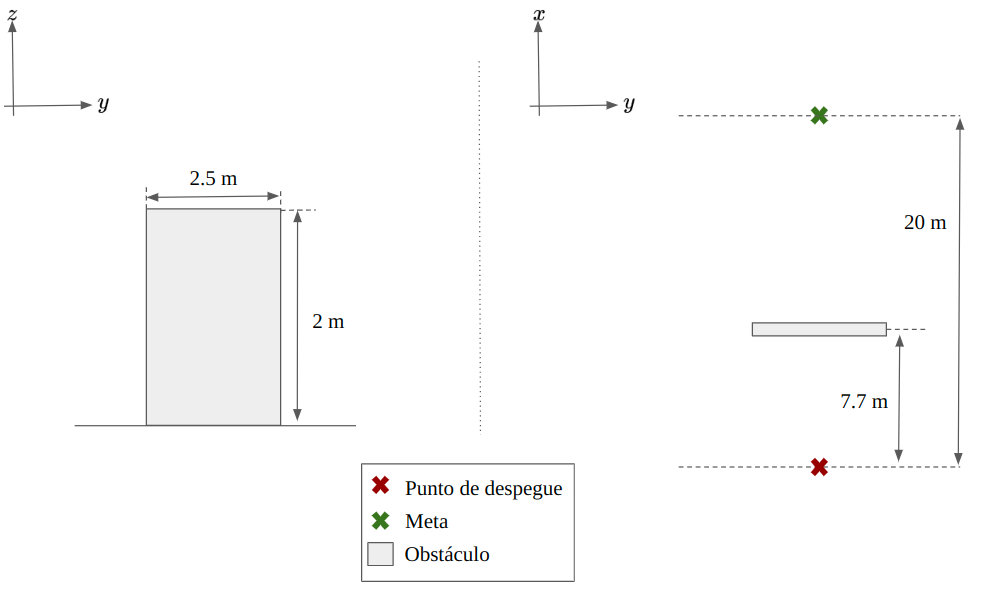
\includegraphics[scale=0.35]{partes/ImgJoao/config-1-single.png}
    \caption[Primera configuración de obstáculos dentro del entorno de AirSim.]{Primera configuración de obstáculos dentro del entorno de AirSim. Obstáculo simple.}
    \label{fig:config-1-single}
\end{figure}

El comportamiento del algoritmo se mostró capaz de evadir el obstáculo de forma robusta, en concreto, de 10 vuelos ejecutados, 10 resultaron en vuelos sin colisión. La figura \ref{fig:single-graph} muestra una visualización desde arriba hacia abajo de camino resultante de seguir las trayectorias generadas por el algoritmo durante un vuelo. Todos vuelos realizados en esta configuración muestran un comportamiento similar al que muestra en la figura \ref{fig:single-graph}, esto es, esquivar el obstáculo hacia la dirección \jim{-y_B}\footnote{Donde \jim{B} es el marco de referencia del cuerpo del QUAV.} y dirigirse hacia la meta una vez no es visible el obstáculo.

\begin{figure}[H]
    \centering
    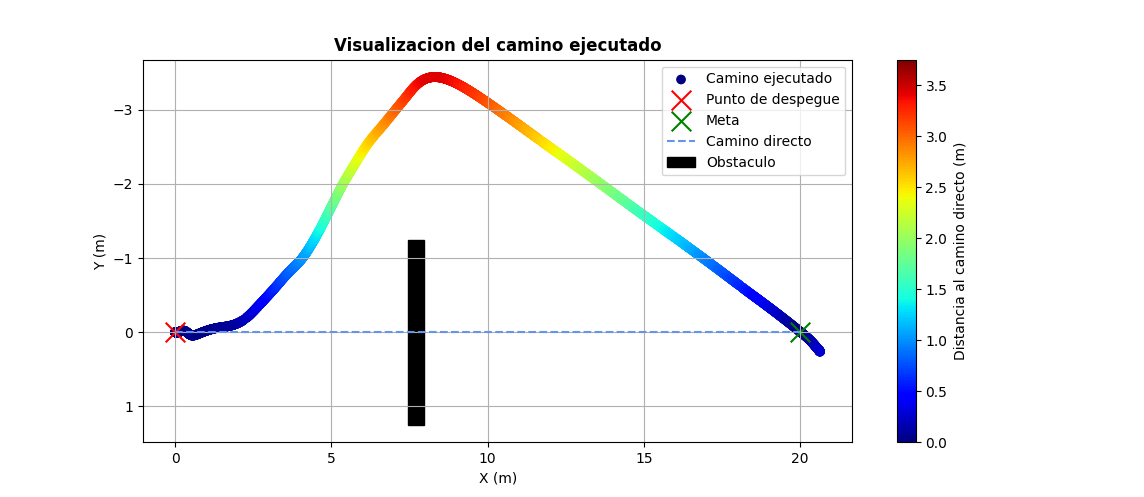
\includegraphics[scale=0.55]{partes/ImgJoao/sim-simgle-panel-graph.png}
    \caption[Visualización del camino ejecutado dentro de la primera configuración de obstáculos.]{Visualización del camino ejecutado dentro de la primera configuración de obstáculos. De 10 vuelos ejecutados dentro de esta configuración, 10 resultaron sin colisión.}
    \label{fig:single-graph}
\end{figure}

La siguiente configuración utilizada es una configuración similar a la anterior pero con un obstáculo adicional también en la misma linea de visión del QUAV. La figura \ref{fig:config-2-double} muestra el diagrama de la segunda configuración.

\begin{figure}[H]
    \centering
    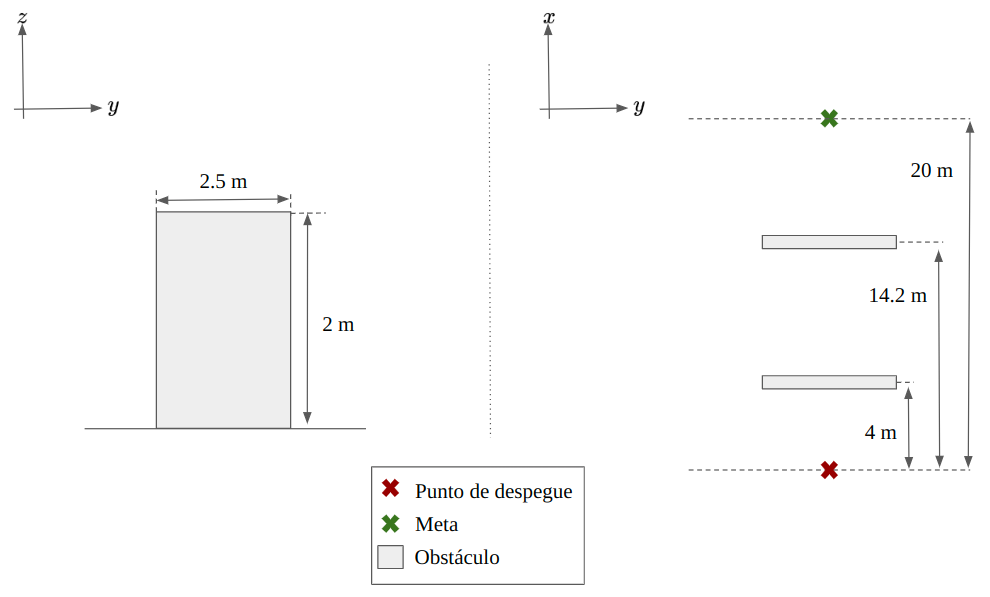
\includegraphics[scale=0.35]{partes/ImgJoao/config-2-double.png}
    \caption[Segunda configuración de obstáculos dentro del entorno de AirSim.]{Segunda configuración de obstáculos dentro del entorno de AirSim. Dos obstáculos consecutivos en la linea de visión del QUAV.}
    \label{fig:config-2-double}
\end{figure}

Tal como en la configuración anterior, el comportamiento de algoritmo fue estable, de 10 vuelos ejecutados, 10 resultaron en vuelos sin colisión. La figura \ref{fig:double-graph} muestra una visualización desde arriba hacia abajo de camino resultante de seguir las trayectorias generadas por el algoritmo durante un vuelo. 

\begin{figure}[H]
    \centering
    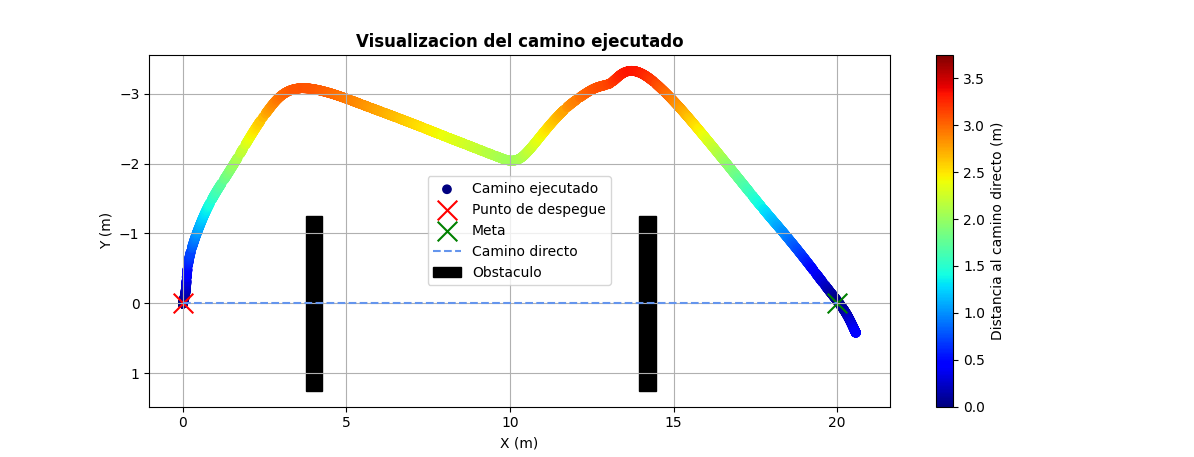
\includegraphics[scale=0.55]{partes/ImgJoao/sim-double-panel-graph.png}
    \caption[Visualización del camino ejecutado dentro de la segunda configuración de obstáculos.]{Visualización del camino ejecutado dentro de la segunda configuración de obstáculos. De 10 vuelos ejecutados dentro de esta configuración, 10 resultaron sin colisión.}
    \label{fig:double-graph}
\end{figure}

Es interesante resaltar, que en los vuelos dentro de la segunda configuración, se confirma el funcionamiento del mecanismo que desactiva la inferencia cuando no hay obstáculos visibles. Para visualizar esto, se desarrolló una visualización 3D que permite visualizar la ejecución del algoritmo incluyendo la información sensorial de profundidad y las trayectorias generadas. En esta visualización se muestra:

\begin{itemize}
    \item La nube de puntos del entorno percibido por las cámaras estereoscópicas del QUAV, el color de los puntos indica la profundidad con respecto al sistema de cámaras, mientras mas rojo mas cerca y mientras mas azul mas lejos.
    \item El camino ejecutado por el QUAV, que se muestra como una curva de color blanco.
    \item La trayectoria mas reciente generada por la política estudiante, que se muestra como una curva de color verde que comienza en la posición en donde se realizo la inferencia.
    \item El radio de colisión del QUAV, que se muestra como una circunferencia de color azul alrededor de la posición del QUAV. Si un obstáculo entra dentro de esta circunferencia se considera una colisión.
    \item La dirección del encabezamiento del QUAV, que se muestra como una linea roja que parte de la posición del QUAV.
    \item Las posiciones de despegue y de meta, que se muestran como un circulo rojo y verde respectivamente.
    \item El camino directo entre el punto de despegue y la meta.
    \item La orientación tridimensional del entorno, que se muestra como 3 flechas; una azul que representa la dirección del eje \jim{z}, una verde que representa la dirección del eje \jim{y} y una roja que representa la dirección del eje \jim{x}. Es importante mencionar que debido a limitaciones del programa de visualización, la dirección del eje \jim{y} se encuentra invertida con respecto al resto de visualizaciones en este capítulo.
\end{itemize}

En las figuras \ref{fig:depth-dual-panel-1}, \ref{fig:depth-dual-panel-2} y \ref{fig:depth-dual-panel-3} se muestran capturas consecutivas de la visualización 3D de un vuelo dentro de la segunda configuración, desde una perspectiva de arriba hacia abajo. En estas figuras podemos observar como solo se generan trayectorias cuando hay un obstáculo cerca en el campo de visión del QUAV.

\begin{figure}[H]
    \centering
    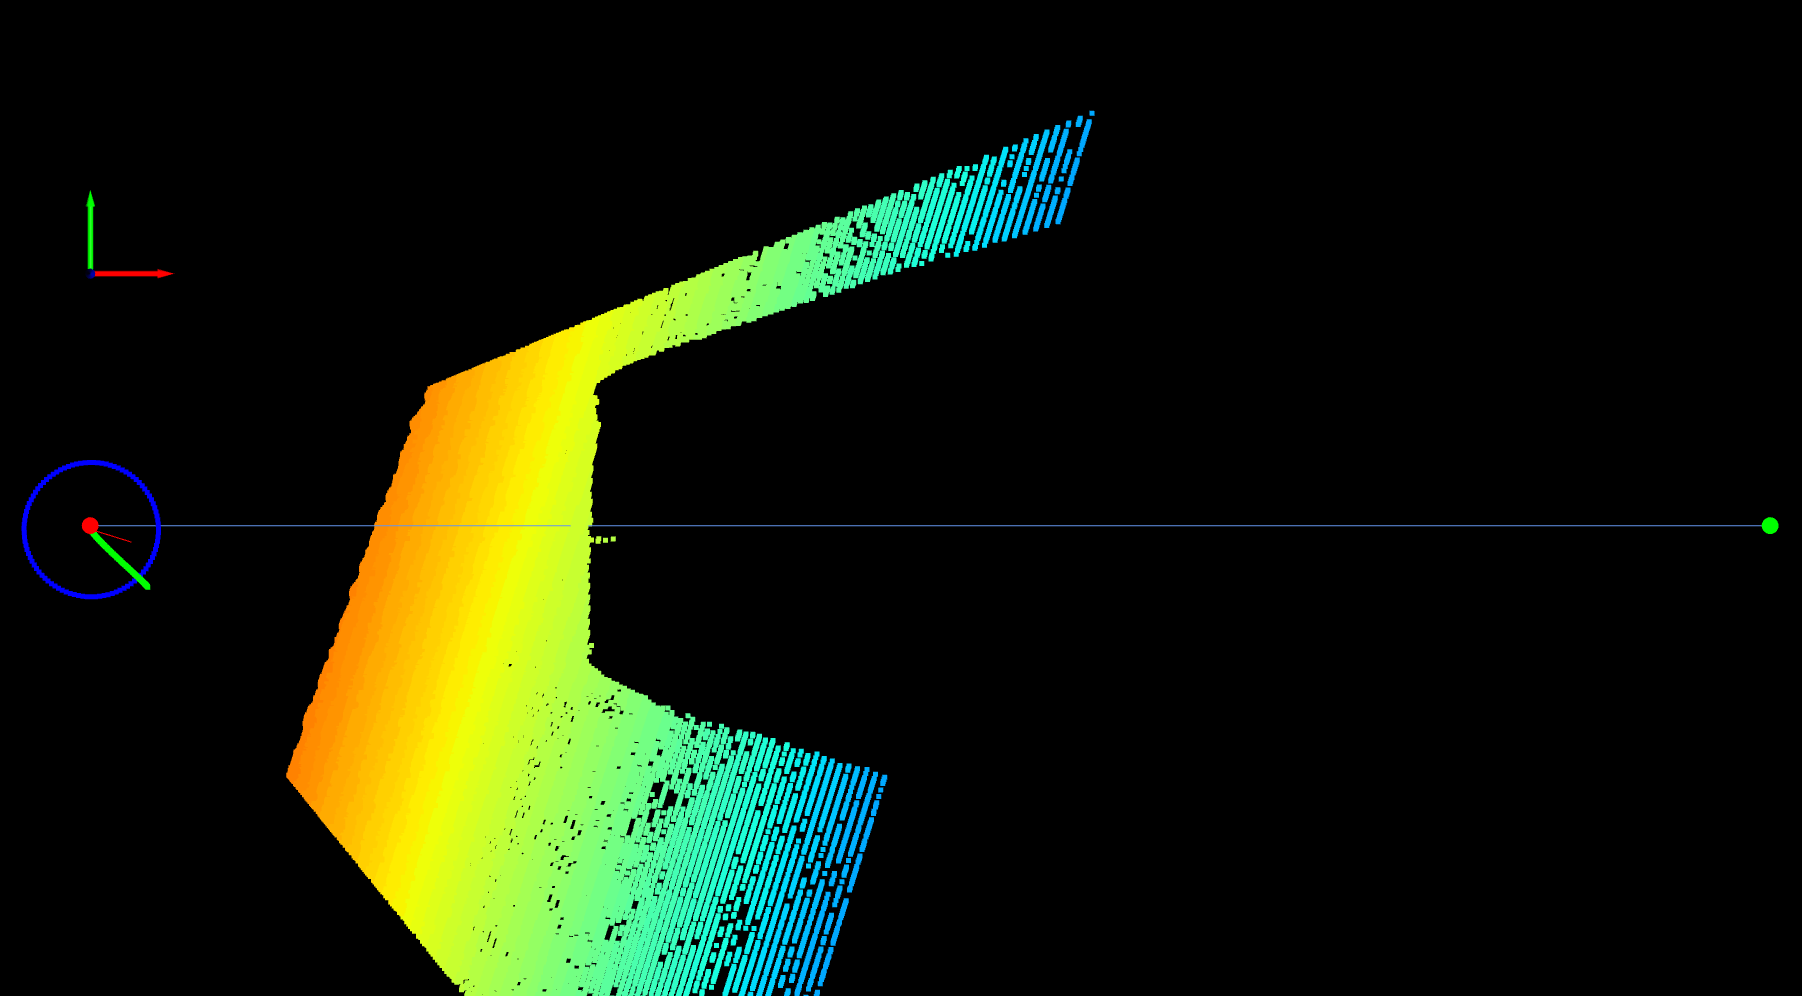
\includegraphics[scale=0.225]{partes/ImgJoao/depth-dual-panel-1-first-obs.png}
    \caption[Visualización del funcionamiento del mecanismo que desactiva la inferencia cuando no hay obstáculos visibles. Inferencia activada, el primer obstáculo está en el campo de visión.]{Visualización del funcionamiento del mecanismo que desactiva la inferencia cuando no hay obstáculos visibles. Inferencia activada, el primer obstáculo está en el campo de visión.}
    \label{fig:depth-dual-panel-1}
\end{figure}

\begin{figure}[H]
    \centering
    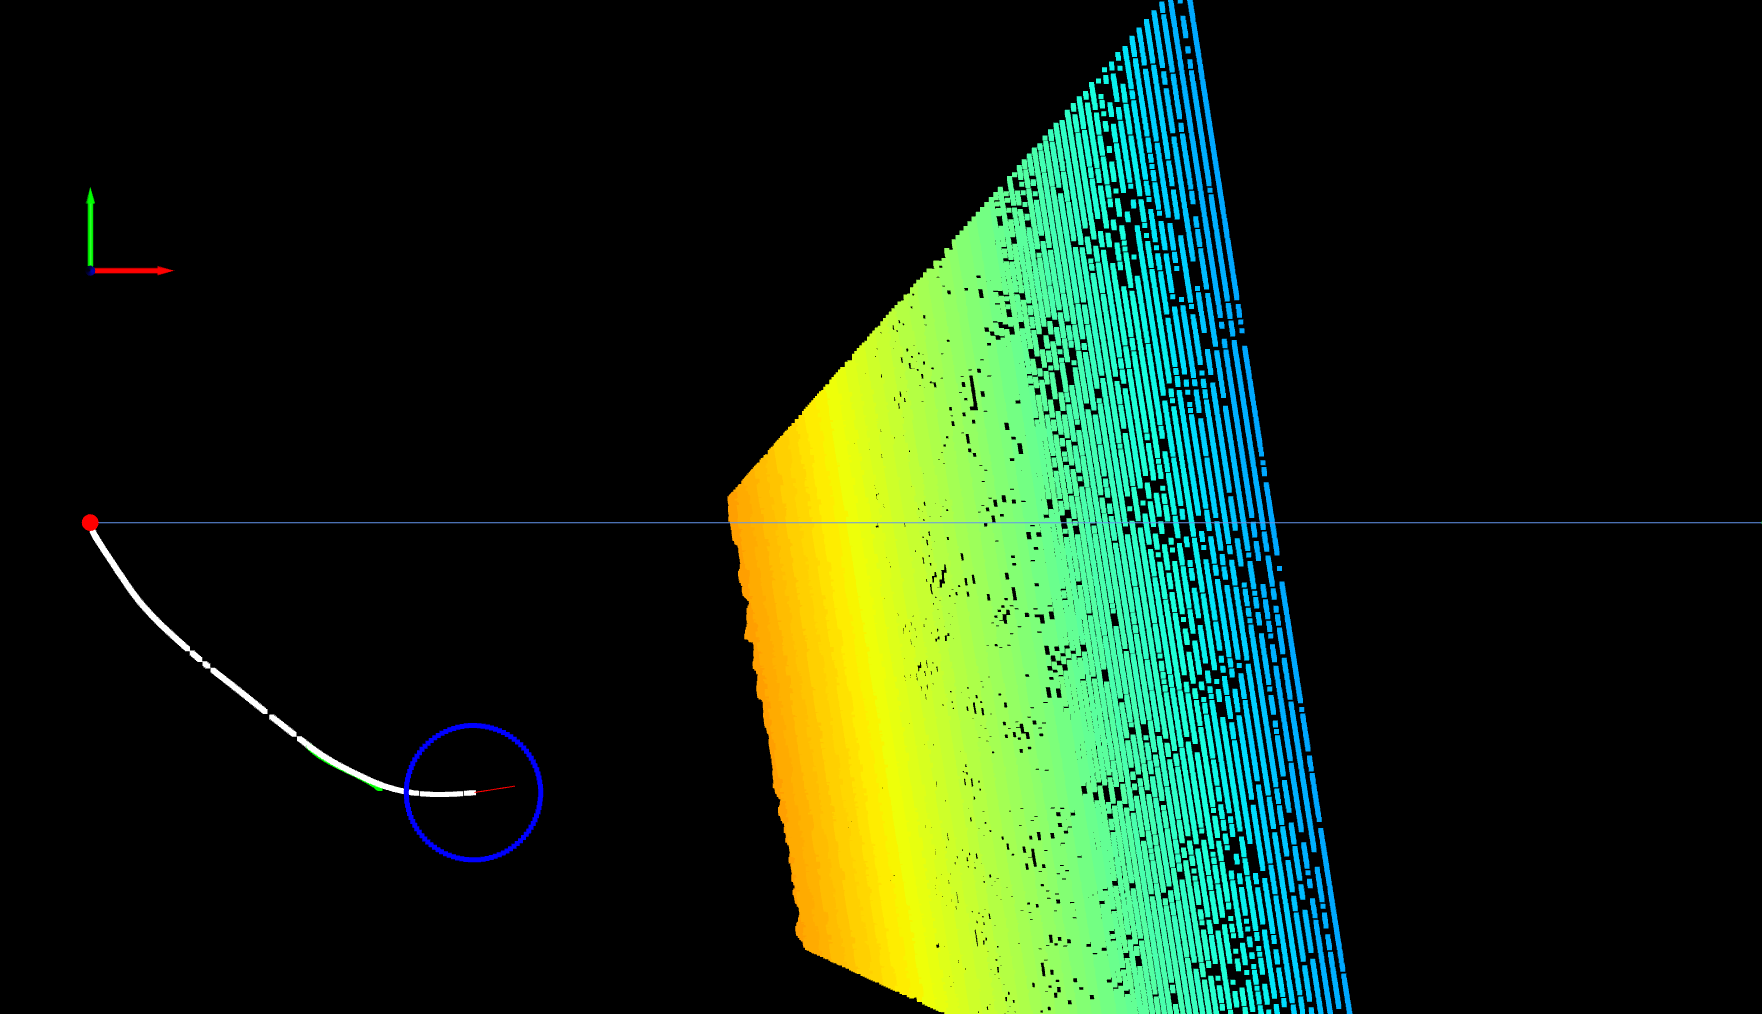
\includegraphics[scale=0.225]{partes/ImgJoao/depth-dual-panel-2-no-obs.png}
    \caption[Visualización del funcionamiento del mecanismo que desactiva la inferencia cuando no hay obstáculos visibles. Inferencia desactivada, no hay obstáculo visible en campo de visión, navegando en dirección a la meta.]{Visualización del funcionamiento del mecanismo que desactiva la inferencia cuando no hay obstáculos visibles. Inferencia desactivada, no hay obstáculo visible en campo de visión, navegando en dirección a la meta.}
    \label{fig:depth-dual-panel-2}
\end{figure}

\begin{figure}[H]
    \centering
    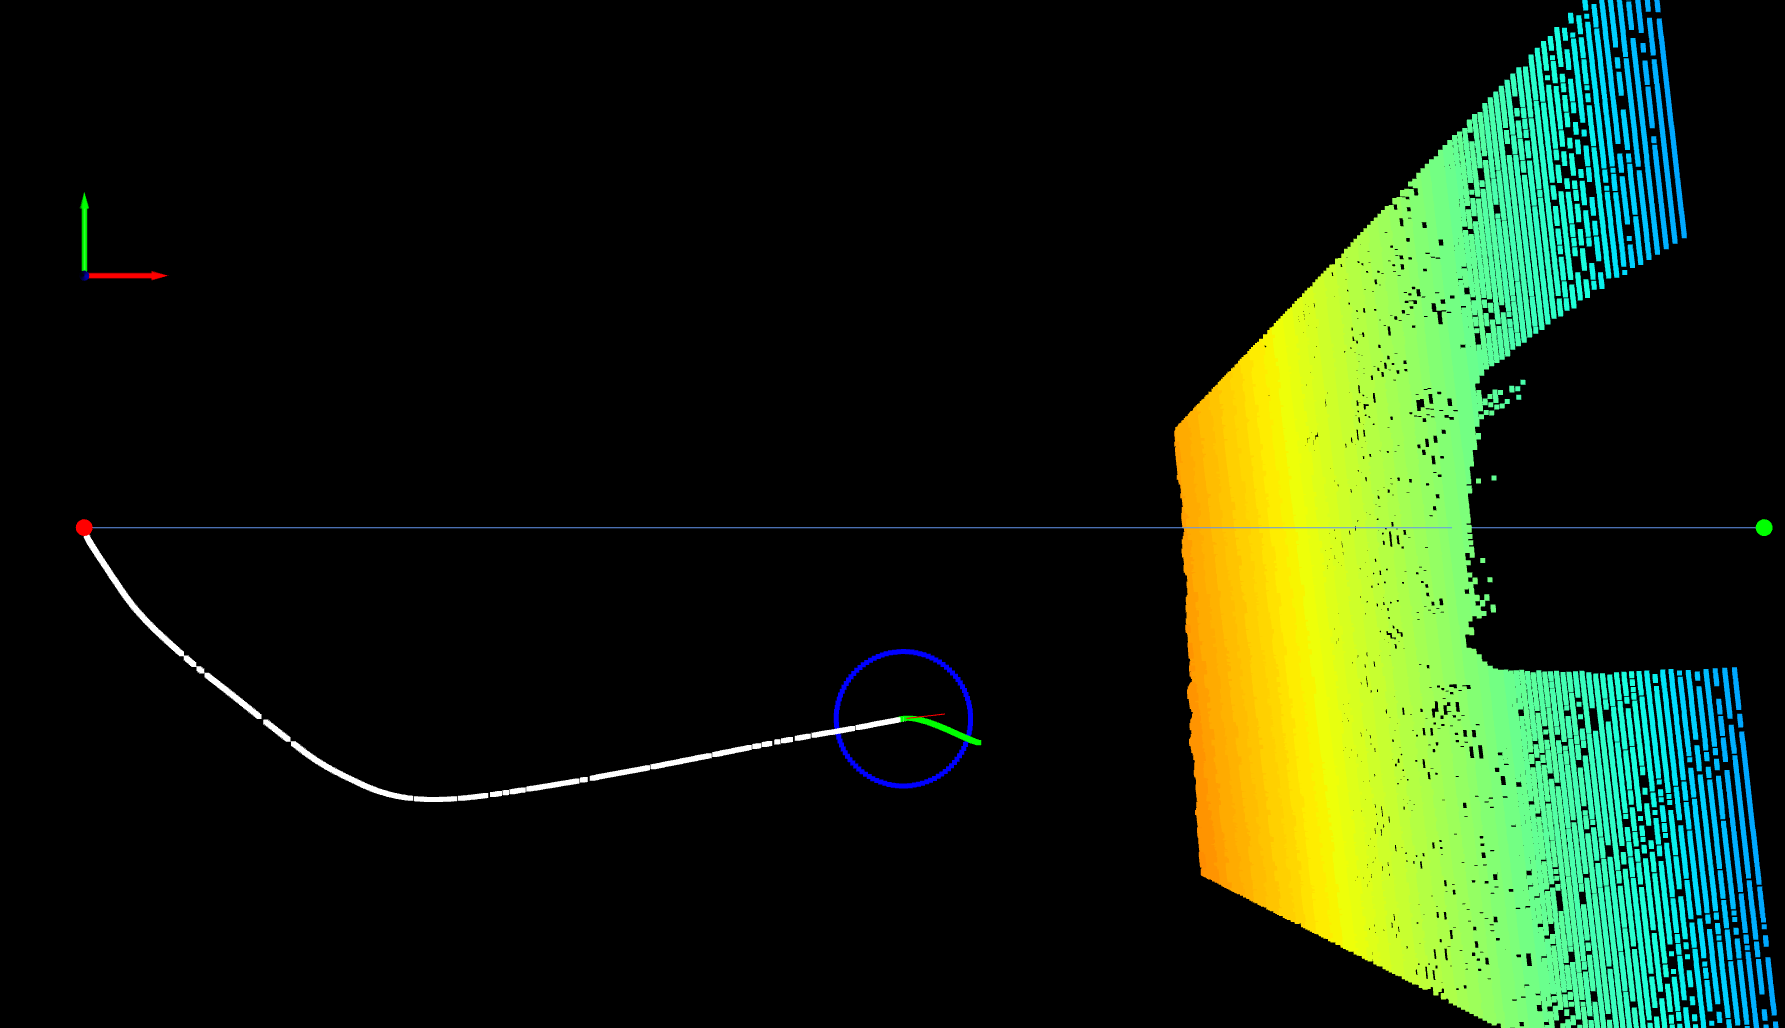
\includegraphics[scale=0.225]{partes/ImgJoao/depth-dual-panel-3-second-obs.png}
    \caption[Visualización del funcionamiento del mecanismo que desactiva la inferencia cuando no hay obstáculos visibles. Inferencia activada, el segundo obstáculo está en el campo de visión.]{Visualización del funcionamiento del mecanismo que desactiva la inferencia cuando no hay obstáculos visibles. Inferencia activada, el segundo obstáculo está en el campo de visión.}
    \label{fig:depth-dual-panel-3}
\end{figure}

Durante todas las pruebas descritas anteriormente, se observó que la política de evasión de obstáculos tiene una preferencia certera a esquivar obstáculos en la dirección \jim{-y_B}, para evaluar este comportamiento el siguiente conjunto de pruebas utiliza una configuración que coloca un obstáculo adicional hacia esa dirección. La figura \ref{fig:config-3-parallel} muestra la tercera configuración utilizada, que consiste de dos obstáculos simples paralelos entre si con una separación de 2 metros.

\begin{figure}[H]
    \centering
    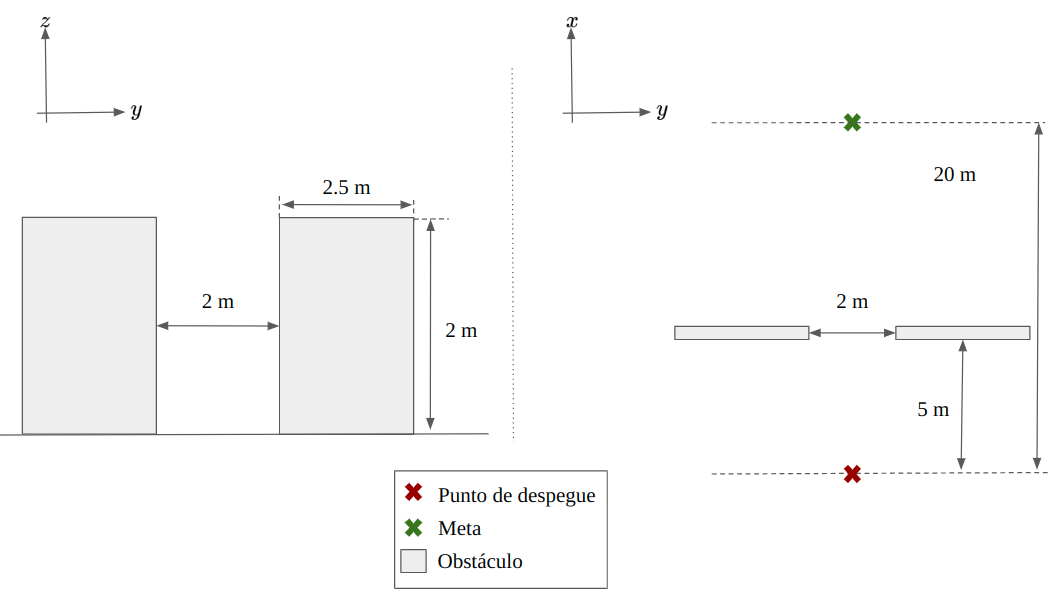
\includegraphics[scale=0.35]{partes/ImgJoao/config-3-parallel.png}
    \caption[Tercera configuración de obstáculos dentro del entorno de AirSim.]{Tercera configuración de obstáculos dentro del entorno de AirSim. Dos obstáculos paralelos con una separación de 2 metros.}
    \label{fig:config-3-parallel}
\end{figure}

Incluso con la presencia de un obstáculo adicional en la dirección \jim{-y_B}, la política de evasión de obstáculos en todas las pruebas realizadas generó trayectorias dirigidas hacia \jim{-y_B}, lo cual produjo colisiones frecuentes, de 10 vuelos ejecutados, 2 fueron sin colisión. En las figuras \ref{fig:depth-parallel-1}, \ref{fig:depth-parallel-2},  \ref{fig:depth-parallel-4} y \ref{fig:depth-parallel-5} se muestran capturas de la visualización 3D de un vuelo que resulto en colisión. Tal como se aprecia en las figuras, mientras ambos obstáculos son visibles en el campo de visión del QUAV, la trayectoria se dirige al espacio entre ambos obstáculos, con un comportamiento que parece guiar al QUAV a una ejecución sin colisiones; sin embargo, en el momento que solo un de los dos obstáculo es visible, en lugar de continuar dirigiéndose hacia el espacio entre ambos obstáculos, la política intenta corregir la trayectoria para esquivar por el flanco en dirección \jim{-y_B} relativo al obstáculo, lo cual produce una colisión. 

\begin{figure}[H]
    \centering
    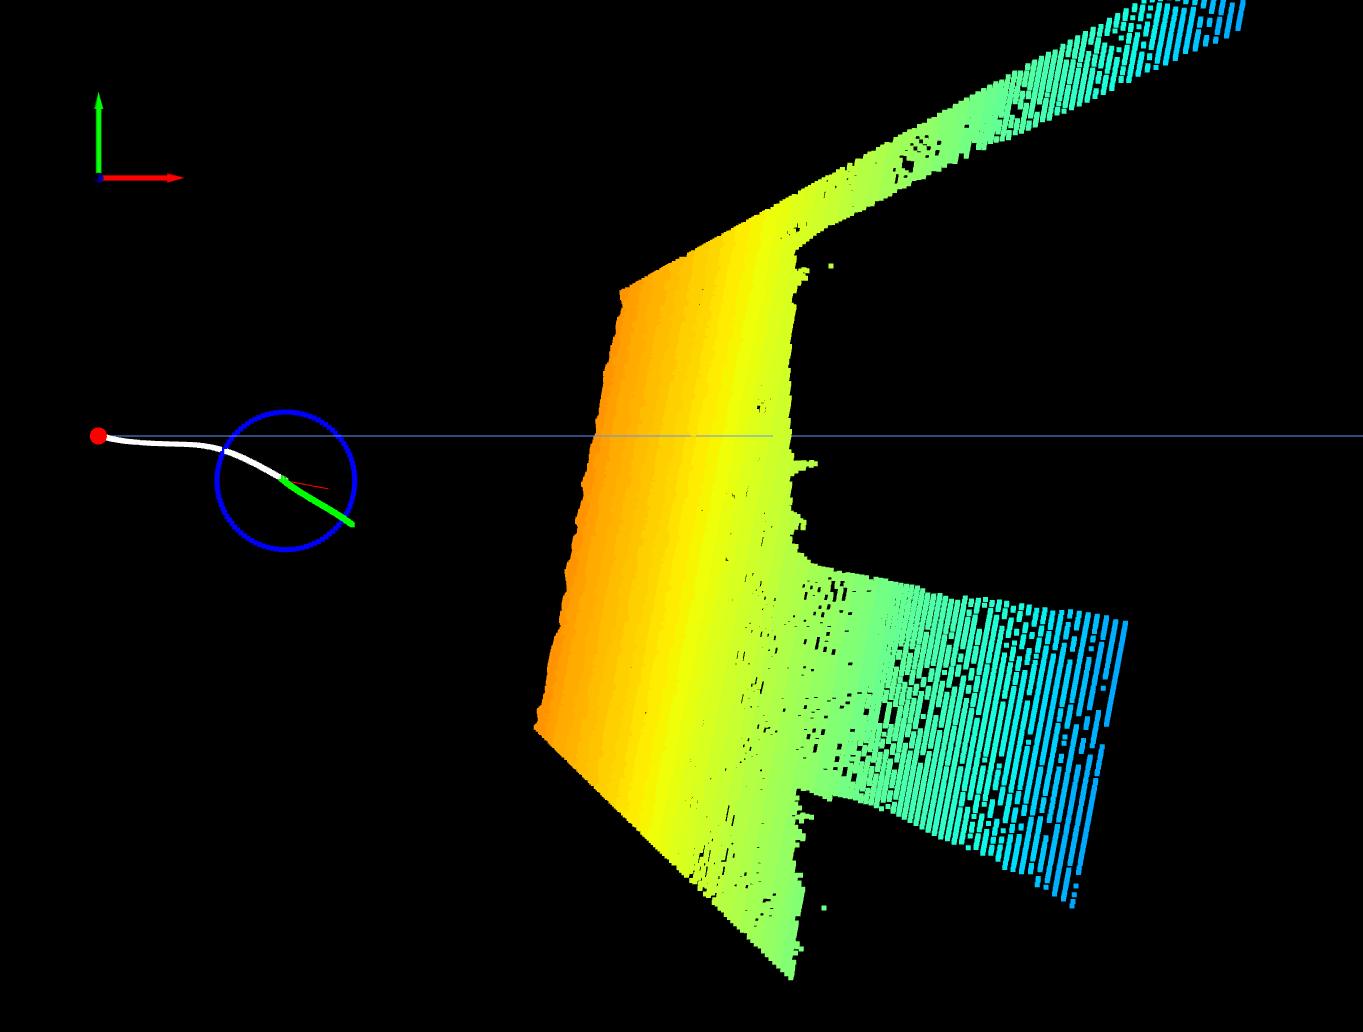
\includegraphics[scale=0.3]{partes/ImgJoao/depth-parallel-1-topdown.png}
    \caption[Visualización 3D de un vuelo en la tercera configuración de obstáculos. Vista de arriba hacia abajo.]{Visualización 3D de un vuelo en la tercera configuración de obstáculos. Vista de arriba hacia abajo. Ambos obstáculos están dentro del campo de visión, las trayectorias generadas se dirigen hacia el espacio entre los obstáculos.}
    \label{fig:depth-parallel-1}
\end{figure}

\begin{figure}[H]
    \centering
    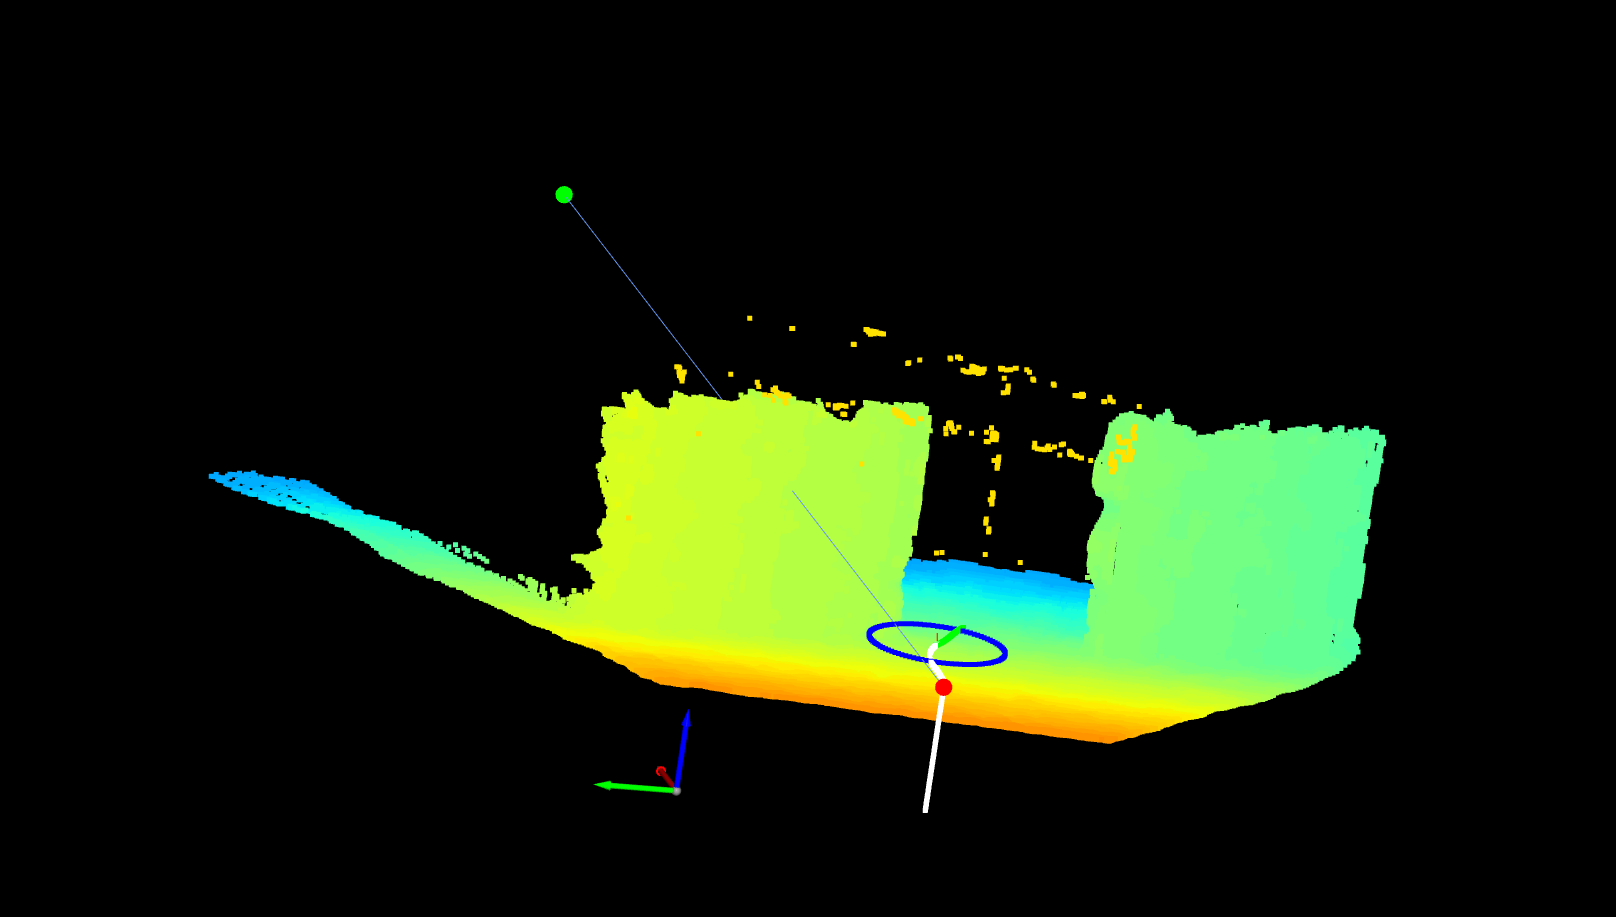
\includegraphics[scale=0.25]{partes/ImgJoao/depth-parallel-2-front.png}
    \caption[Visualización 3D de un vuelo en la tercera configuración de obstáculos. Vista frontal.]{Visualización 3D de un vuelo en la tercera configuración de obstáculos. Vista frontal. Ambos obstáculos están dentro del campo de visión, las trayectorias generadas se dirigen hacia el espacio entre los obstáculos.}
    \label{fig:depth-parallel-2}
\end{figure}

\begin{figure}[H]
    \centering
    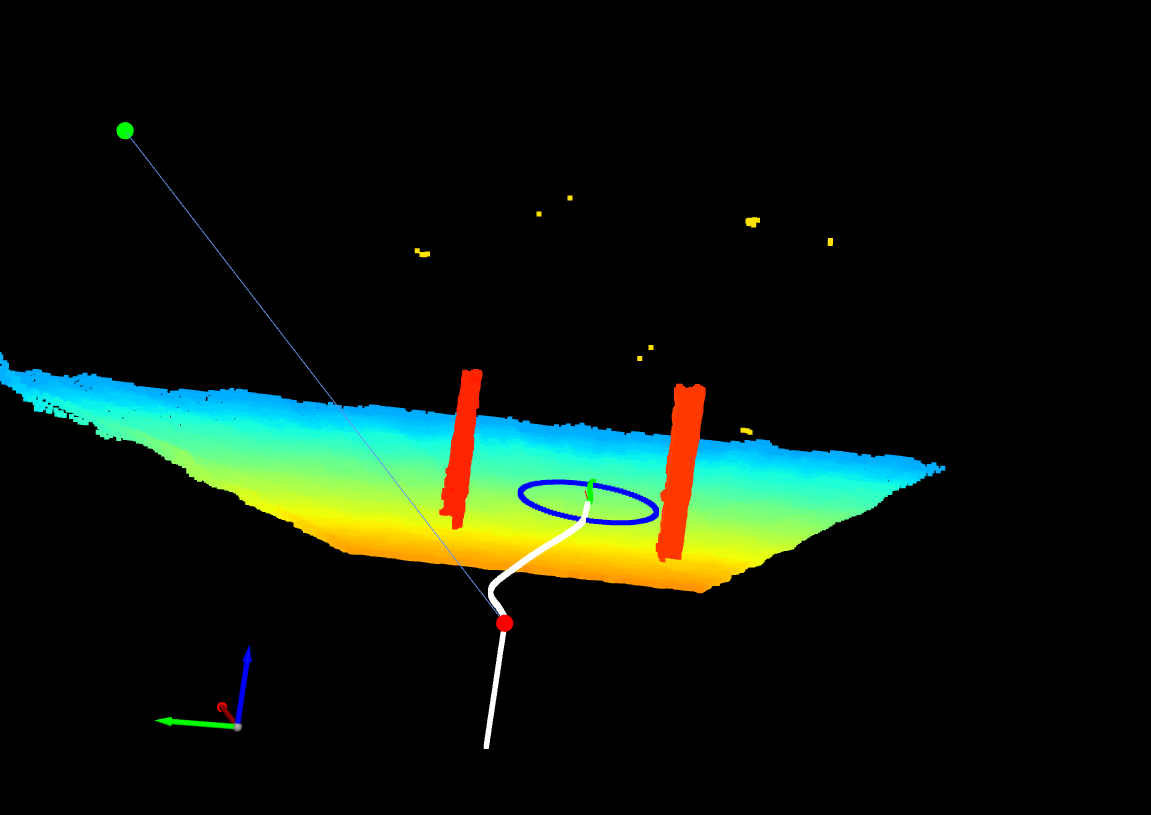
\includegraphics[scale=0.32]{partes/ImgJoao/depth-parallel-4-front-red.png}
    \caption[Visualización 3D de un vuelo en la tercera configuración de obstáculos. Vista frontal. Navegando entre el espacio entre los obstáculos.]{Visualización 3D de un vuelo en la tercera configuración de obstáculos. Vista frontal. Navegando entre el espacio entre los obstáculos. Ambos obstáculos están dentro del campo de visión, las trayectorias generadas se dirigen hacia el espacio entre los obstáculos.}
    \label{fig:depth-parallel-4}
\end{figure}

\begin{figure}[H]
    \centering
    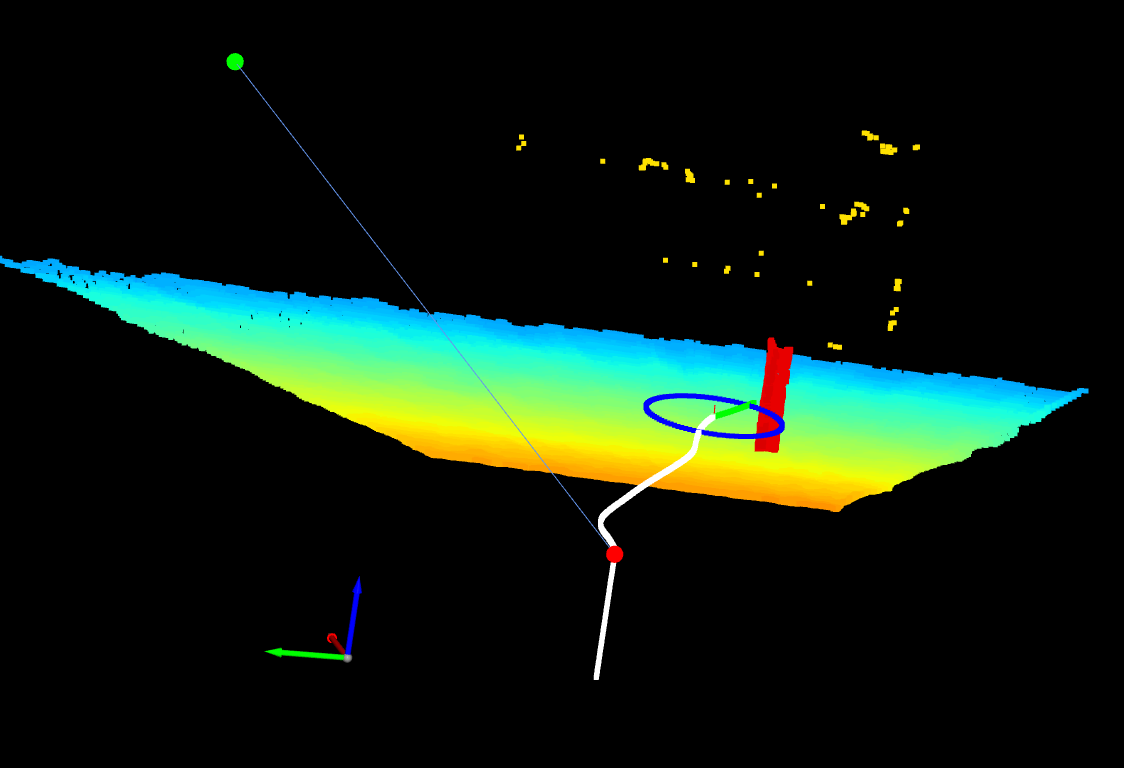
\includegraphics[scale=0.32]{partes/ImgJoao/depth-parallel-5-front-collision.png}
    \caption[Visualización 3D de un vuelo en la tercera configuración de obstáculos. Vista frontal. Colisión.]{Visualización 3D de un vuelo en la tercera configuración de obstáculos. Vista frontal. En el momento que uno de los dos obstáculos desaparece del campo de visión, en lugar de continuar dirigiéndose hacia el espacio entre ambos obstáculos, la política intenta corregir la trayectoria para esquivar por el flanco en dirección \jim{-y_B} relativo al obstáculo, lo cual produce una colisión. }
    \label{fig:depth-parallel-5}
\end{figure}


Para evaluar esta preferencia fuerte a esquivar por el flanco en la dirección \jim{-y_B} con respecto al obstáculo, la siguiente configuración a evaluar es de tal forma que no existe una forma de esquivar por el flanco en la dirección \jim{-y_B} sin regresar hacia atrás, la figura \ref{fig:config-4-wall} muestra un diagrama de la configuración en cuestión.

\begin{figure}[H]
    \centering
    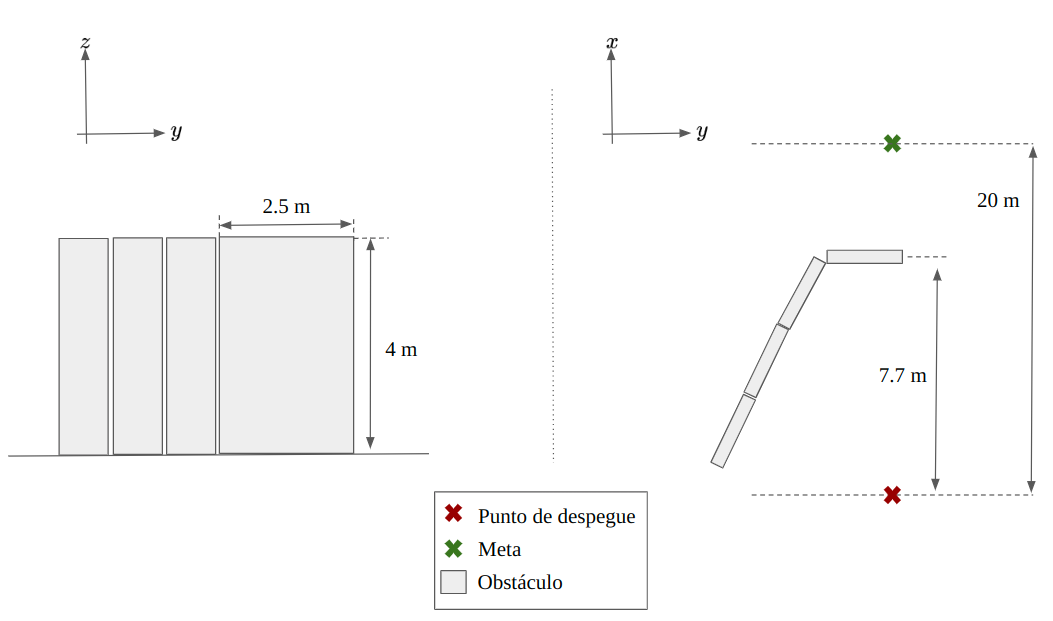
\includegraphics[scale=0.35]{partes/ImgJoao/config-4-left-wall.png}
    \caption[Cuarta configuración de obstáculos dentro del entorno de AirSim.]{Cuarta configuración de obstáculos dentro del entorno de AirSim. Obstáculo simple con pared del lado izquierdo.}
    \label{fig:config-4-wall}
\end{figure}

Todos los vuelos realizados en esta configuración terminaron en una colisión. Las figuras \ref{depth-wall-1}, \ref{depth-wall-2}, \ref{depth-wall-3}, \ref{depth-wall-4} y \ref{depth-wall-5} muestran capturas de la visualización 3D de un vuelo en esta configuración que resulto en colisión. En las figuras se observa como la política de evasión de obstáculos intenta generar trayectorias que se dirigen hacia la región en la dirección \jim{-y_B} en donde no hay información de profundidad, probablemente esperando encontrar el borde del obstáculo en esa dirección, pero como en esta configuración de obstáculos ese borde se encuentra hacia atrás, se produce una colisión.

\begin{figure}[H]
    \centering
    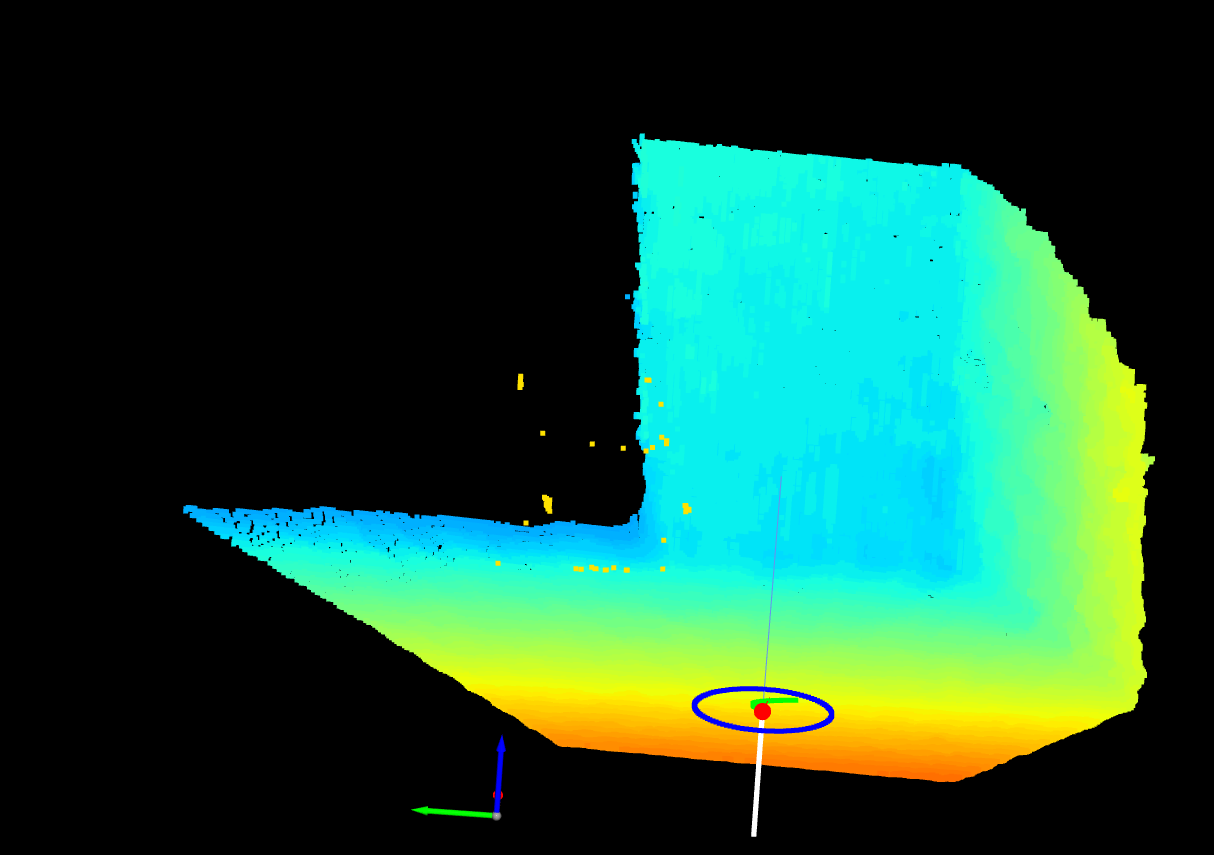
\includegraphics[scale=0.23]{partes/ImgJoao/depth-wall-1-front.png}
    \caption[Visualización 3D de un vuelo en la cuarta configuración de obstáculos. Vista frontal.]{Visualización 3D de un vuelo en la cuarta configuración de obstáculos. Vista frontal.}
    \label{depth-wall-1}
\end{figure}

\begin{figure}[H]
    \centering
    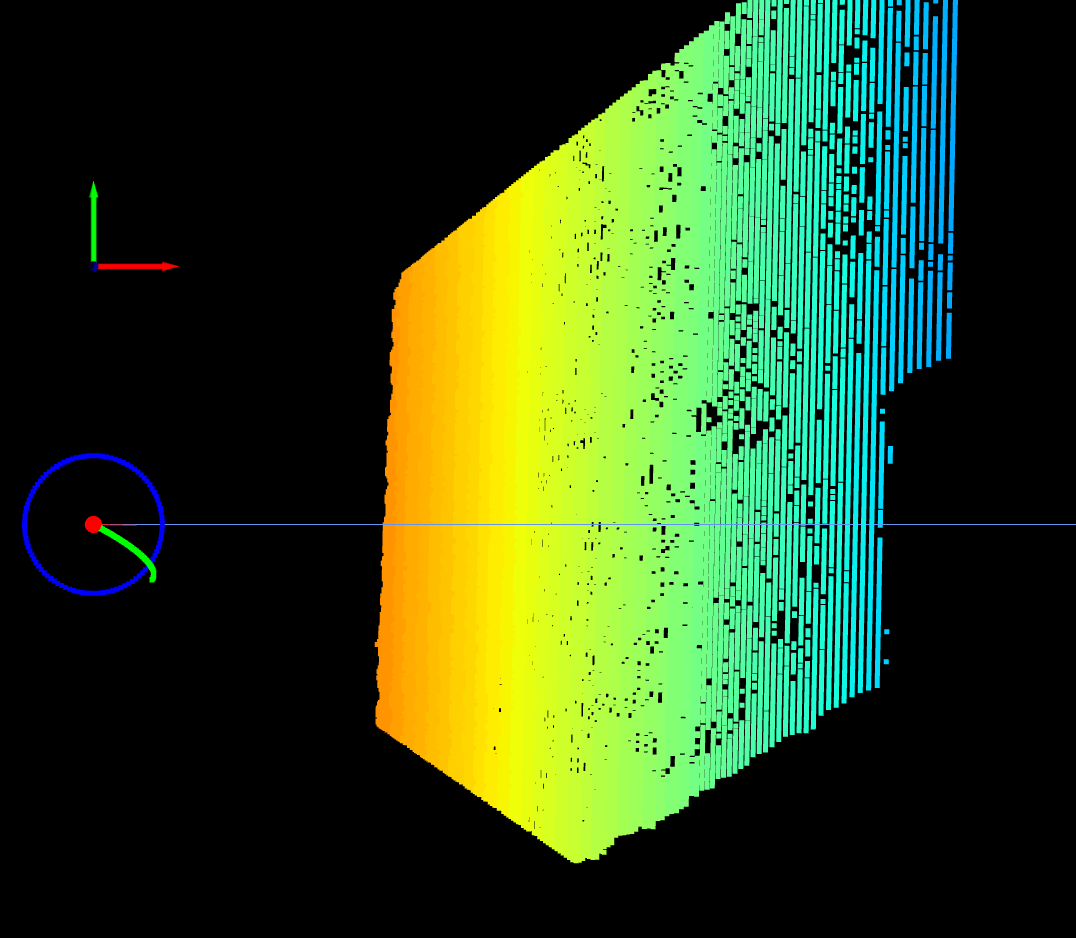
\includegraphics[scale=0.25]{partes/ImgJoao/depth-wall-2-top.png}
    \caption[Visualización 3D de un vuelo en la cuarta configuración de obstáculos. Vista de arriba hacia abajo. Búsqueda del borde del obstáculo (1).]{Visualización 3D de un vuelo en la cuarta configuración de obstáculos. Vista de arriba hacia abajo. Las trayectorias se dirigen hacia la región en dirección \jim{-y_B} sin información de profundidad, probablemente buscando el borde del obstáculo.}
    \label{depth-wall-2}
\end{figure}

\begin{figure}[H]
    \centering
    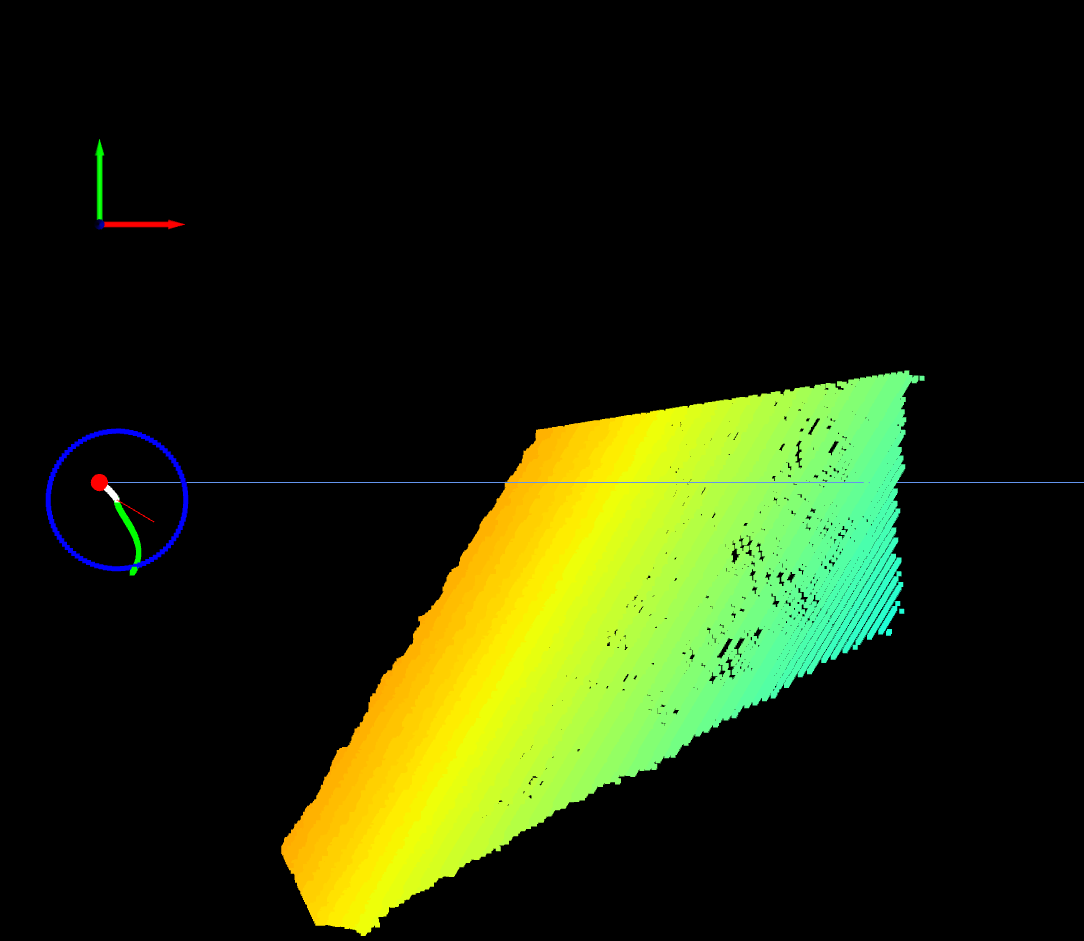
\includegraphics[scale=0.25]{partes/ImgJoao/depth-wall-3-try-arround.png}
    \caption[Visualización 3D de un vuelo en la cuarta configuración de obstáculos. Vista de arriba hacia abajo. Búsqueda del borde del obstáculo (2).]{Visualización 3D de un vuelo en la cuarta configuración de obstáculos. Vista de arriba hacia abajo. Las trayectorias continúan dirigiéndose hacia la región en dirección \jim{-y_B} sin información de profundidad, probablemente buscando el borde del obstáculo.}
    \label{depth-wall-3}
\end{figure}

\begin{figure}[H]
    \centering
    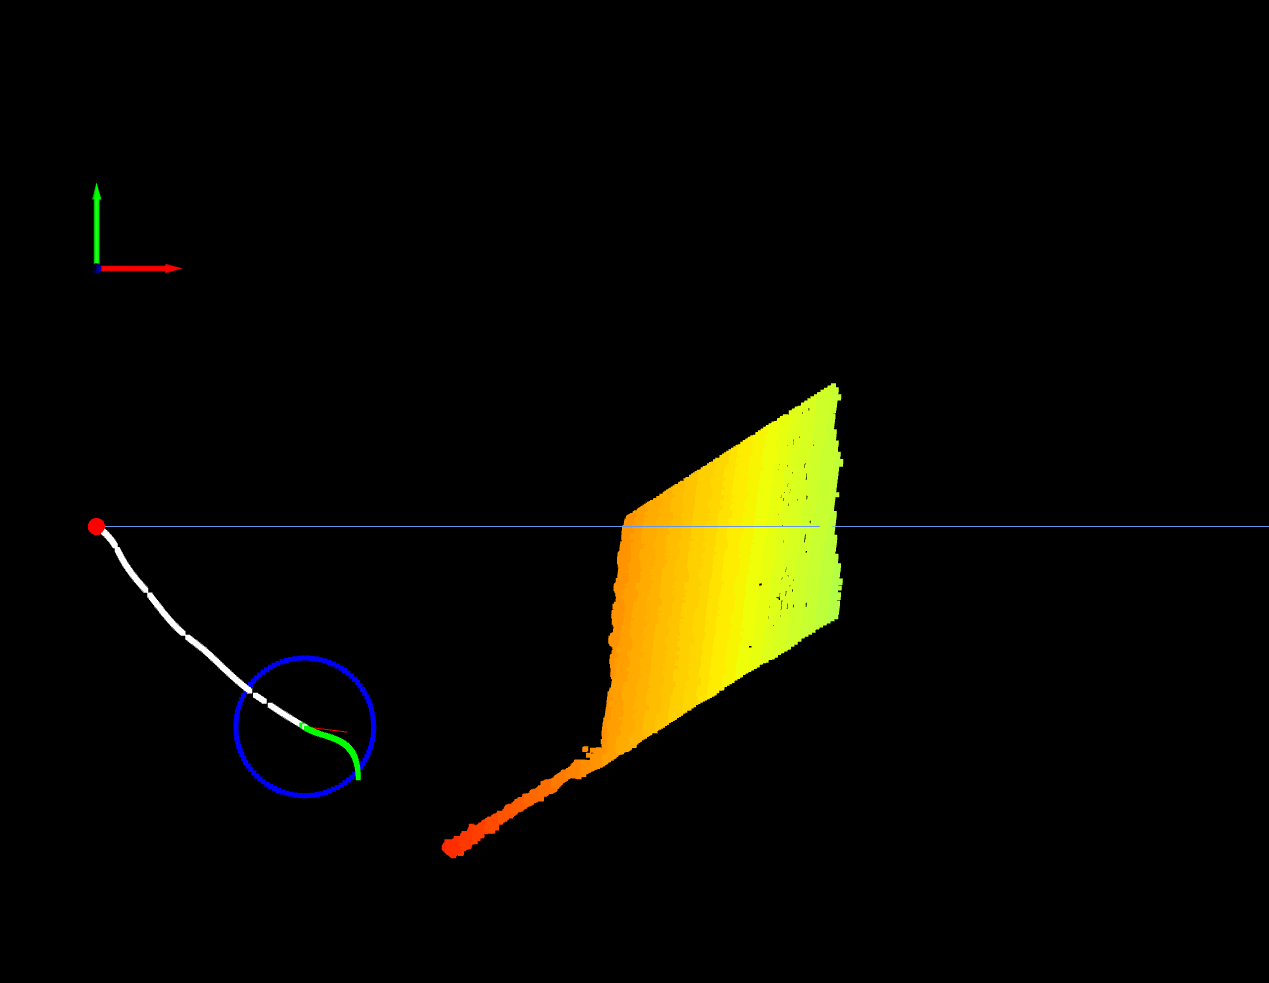
\includegraphics[scale=0.25]{partes/ImgJoao/depth-wall-4-still-go-arround.png}
    \caption[Visualización 3D de un vuelo en la cuarta configuración de obstáculos. Vista de arriba hacia abajo. Búsqueda del borde del obstáculo (3).]{Visualización 3D de un vuelo en la cuarta configuración de obstáculos. Vista de arriba hacia abajo. Las trayectorias continúan dirigiéndose hacia la región en dirección \jim{-y_B} sin información de profundidad, probablemente buscando el borde del obstáculo.}
    \label{depth-wall-4}
\end{figure}

\begin{figure}[H]
    \centering
    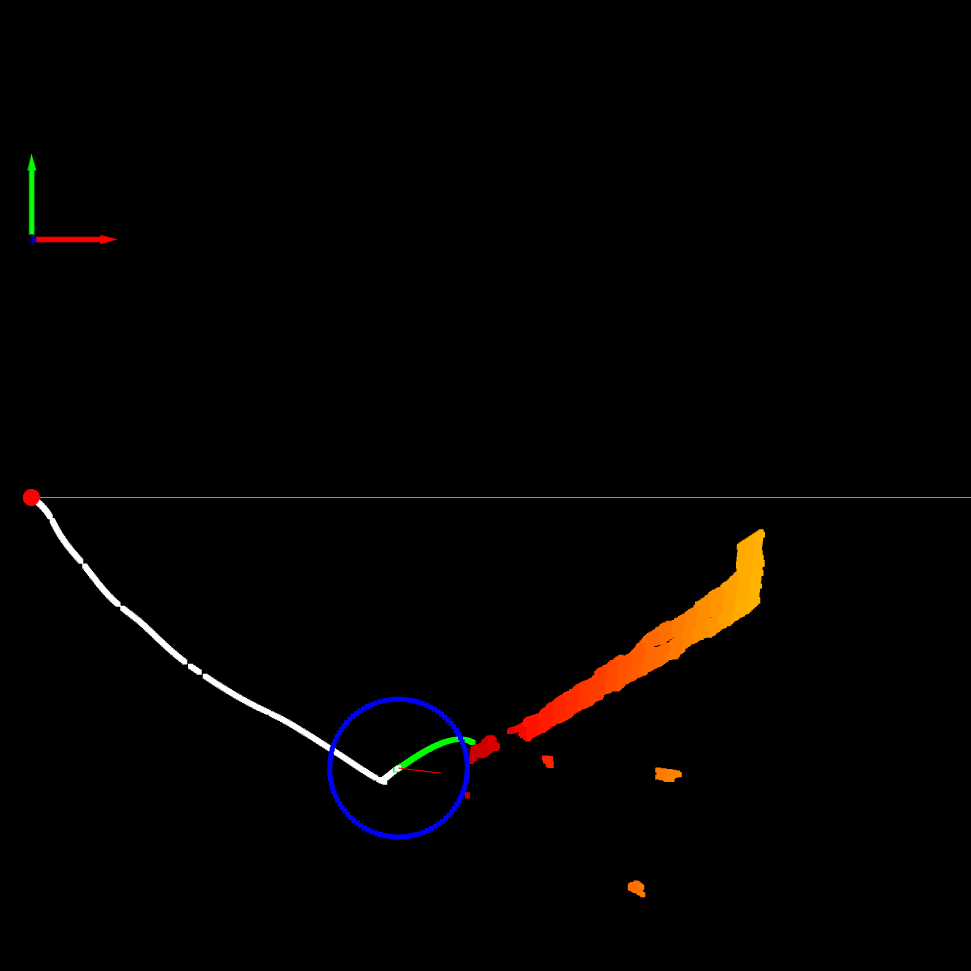
\includegraphics[scale=0.25]{partes/ImgJoao/depth-wall-5-crash.png}
    \caption[Visualización 3D de un vuelo en la cuarta configuración de obstáculos. Vista de arriba hacia abajo. Colisión.]{Visualización 3D de un vuelo en la cuarta configuración de obstáculos. Vista de arriba hacia abajo. Al no conseguir el borde del obstáculo a tiempo, se produce una colisión.}
    \label{depth-wall-5}
\end{figure}

De estos resultados se confirma que los efectos consecuencia de las dificultades encontradas durante el refinamiento fino de la política estudiante son la preferencia certera a esquivar obstáculos hacia el flanco izquierdo (en dirección \jim{-y_B}), y que estos efectos producen colisiones en configuraciones de obstáculos donde no es posible esquivar hacia ese flanco.

En la tabla \ref{table:sim-results} se muestra un resumen de los resultados obtenidos en los vuelos en simulación. En esta tabla se muestra que la política es estable para las configuraciones de obstáculos donde es trivial esquivar por el flanco izquierdo. De igual forma, se muestra que la política es inestable y propensa a producir colisiones para las configuraciones de obstáculos donde es no trivial esquivar por el flanco izquierdo.

\begin{table}[h]
\centering
\begin{tabular}{||c || c | c | c||} 
 \hline
 \textbf{Configuración} & \jim{N_{total}} & \jim{N_{exito}} & \textbf{porcentaje de éxito} \\ [0.5ex] 
 \hline\hline
 Obstáculo simple              & 10 & 10 & 100\% \\ 
 \hline
 Dos obstáculos consecutivos   & 10 & 10 & 100\% \\
 \hline
 Dos obstáculos paralelos      & 10 & 2  & 20 \% \\
 \hline
 Obstáculo con pared izquierda & 10 & 0  & 0  \% \\
 \hline
\end{tabular}
\caption[Resumen de los resultados obtenidos en los vuelos en simulación.]{Resumen de los resultados obtenidos en los vuelos en simulación. \jim{N_{total}} y \jim{N_{exito}} son el numero de vuelos totales y sin colisión respectivamente.}
\label{table:sim-results}
\end{table}

\subsection{Vuelos sobre la plataforma física}

\label{sec:results-SOTEN}

En esta sección se describen las configuraciones y resultados de los vuelos realizados sobre la plataforma física de implementación (QUAV SOTEN\footnote{En la figura \ref{fig:SOTEN} se muestra al QUAV SOTEN.}) en un entorno de la vida real. Esto vuelos fueron ejecutados en un campo de vuelo para drones ubicado en la prefectura de Chiba, Japón; las condiciones climáticas del día fueron: soleado con un ligero viento en dirección hacia el oeste. Durante los vuelos, un piloto experto estuvo preparado para controlar manualmente el QUAV en caso de que una colisión fuera inminente. En esta sección se utilizara el termino ``colision'' para referirse al evento de interrumpir el vuelo autónomo para evitar una colisión inminente.

La primera configuración de obstáculos utilizada fue una configuración simple con un solo obstáculo en la linea directa de visión del QUAV, la figura \ref{real-1-single-0-setup} muestra una fotografía ilustrada que describe la configuración.

\begin{figure}[H]
    \centering
    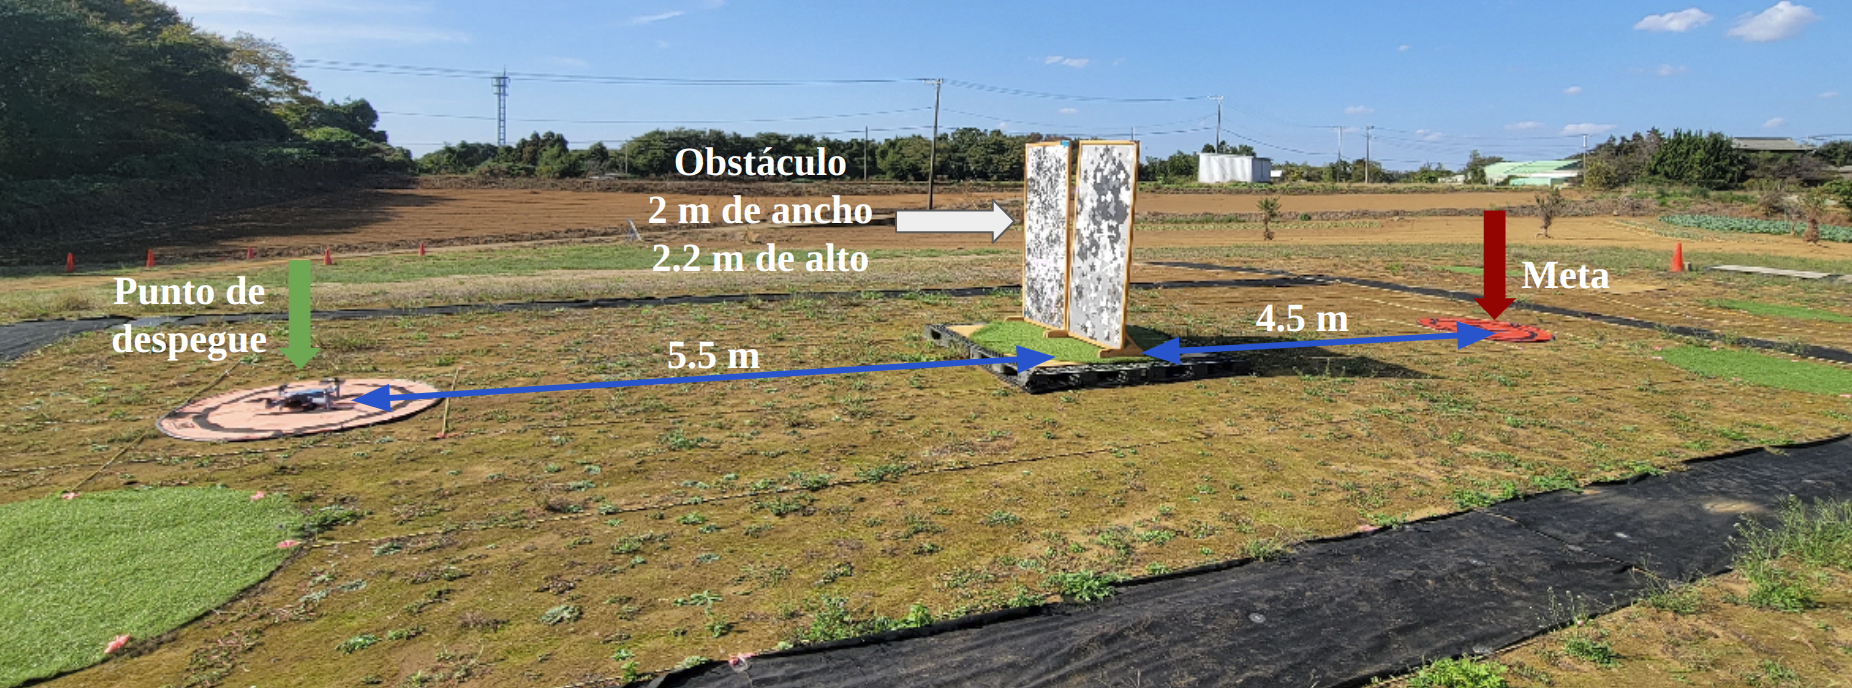
\includegraphics[scale=0.22]{partes/ImgJoao/real-1-single-0-setup.png}
    \caption[Configuración de obstáculos en entorno real: Obstáculo simple]{Configuración de obstáculos en entorno real: Obstáculo simple.}
    \label{real-1-single-0-setup}
\end{figure}

Se realizaron 11 vuelos en esta configuración, y los resultados fueron análogos a los obtenidos en simulación, en concreto, de 11 vuelos ejecutados, 10 resultaron sin colisión. Los caminos resultantes de los vuelos también fueron análogos a los obtenidos en simulación, sin embargo, debido a variaciones en el viento y en las condiciones de iluminación, algunas ejecuciones se desviaron considerablemente del camino directo. La figura \ref{real-1-single-2-graph-worst} muestra una visualización del camino resultante del vuelo con \textbf{mayor} desviación; por otro lado la figura \ref{real-1-single-1-graph-best} una visualización del camino resultante del vuelo con \textbf{menor} desviación; tal como se aprecia en las figuras, la desviación máxima durante el vuelo estuvo contenida entre 2 metros y 4 metros a lo largo de los vuelos ejecutados.

\begin{figure}[H]
    \centering
    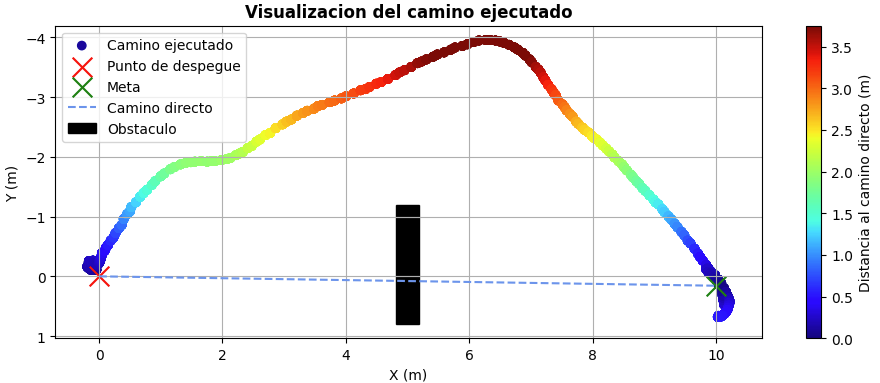
\includegraphics[scale=0.47]{partes/ImgJoao/real-1-single-2-graph-worst.png}
    \caption[Visualización del camino resultante del vuelo con mayor desviación para un obstáculo simple en entorno real.]{Visualización del camino resultante del vuelo con \textbf{mayor} desviación para un obstáculo simple en entorno real.}
    \label{real-1-single-2-graph-worst}
\end{figure}

\begin{figure}[H]
    \centering
    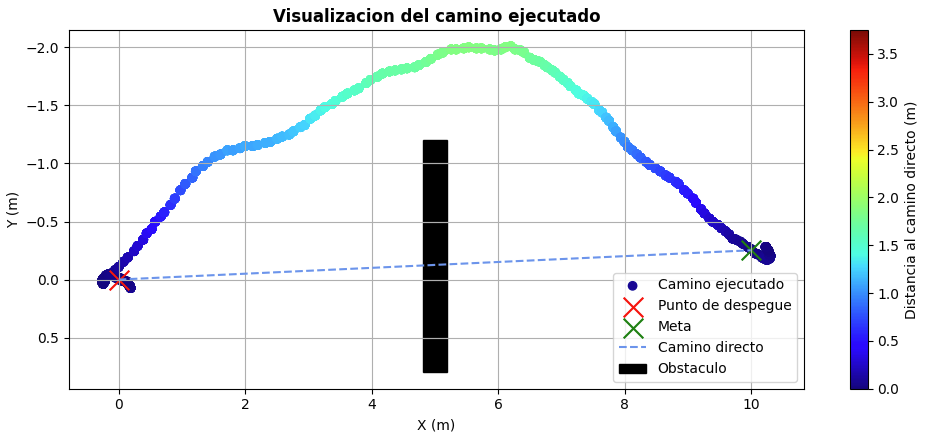
\includegraphics[scale=0.47]{partes/ImgJoao/real-1-single-1-graph-best.png}
    \caption[Visualización del camino resultante del vuelo con menor desviación para un obstáculo simple en entorno real.]{Visualización del camino resultante del vuelo con \textbf{menor} desviación para un obstáculo simple en entorno real.}
    \label{real-1-single-1-graph-best}
\end{figure}

En todos los vuelos ejecutados en esta configuración, el algoritmo esquivó el obstáculo por el flanco izquierdo y continuo en dirección a la meta. Las figuras \ref{real-1-single-3-frames-1}, \ref{real-1-single-3-frames-2} y \ref{real-1-single-3-frames-3} muestran capturas de una grabación de uno de los vuelos sobre esta configuración. Las figuras \ref{real-1-single-4-frames-1}, \ref{real-1-single-4-frames-2} y \ref{real-1-single-4-frames-3} también muestran capturas de una grabación de uno de los vuelos sobre esta configuración pero en una perspectiva diferente. En estas figuras se aprecia claramente el comportamiento del algoritmo, en particular: comenzar el vuelo, esquivar el obstáculo por el flanco izquierdo, continuar avanzando hasta que se termine la trayectoria actual y finalmente, como no se observan obstáculos, navegar en dirección a la meta.

\begin{figure}[H]
    \centering
    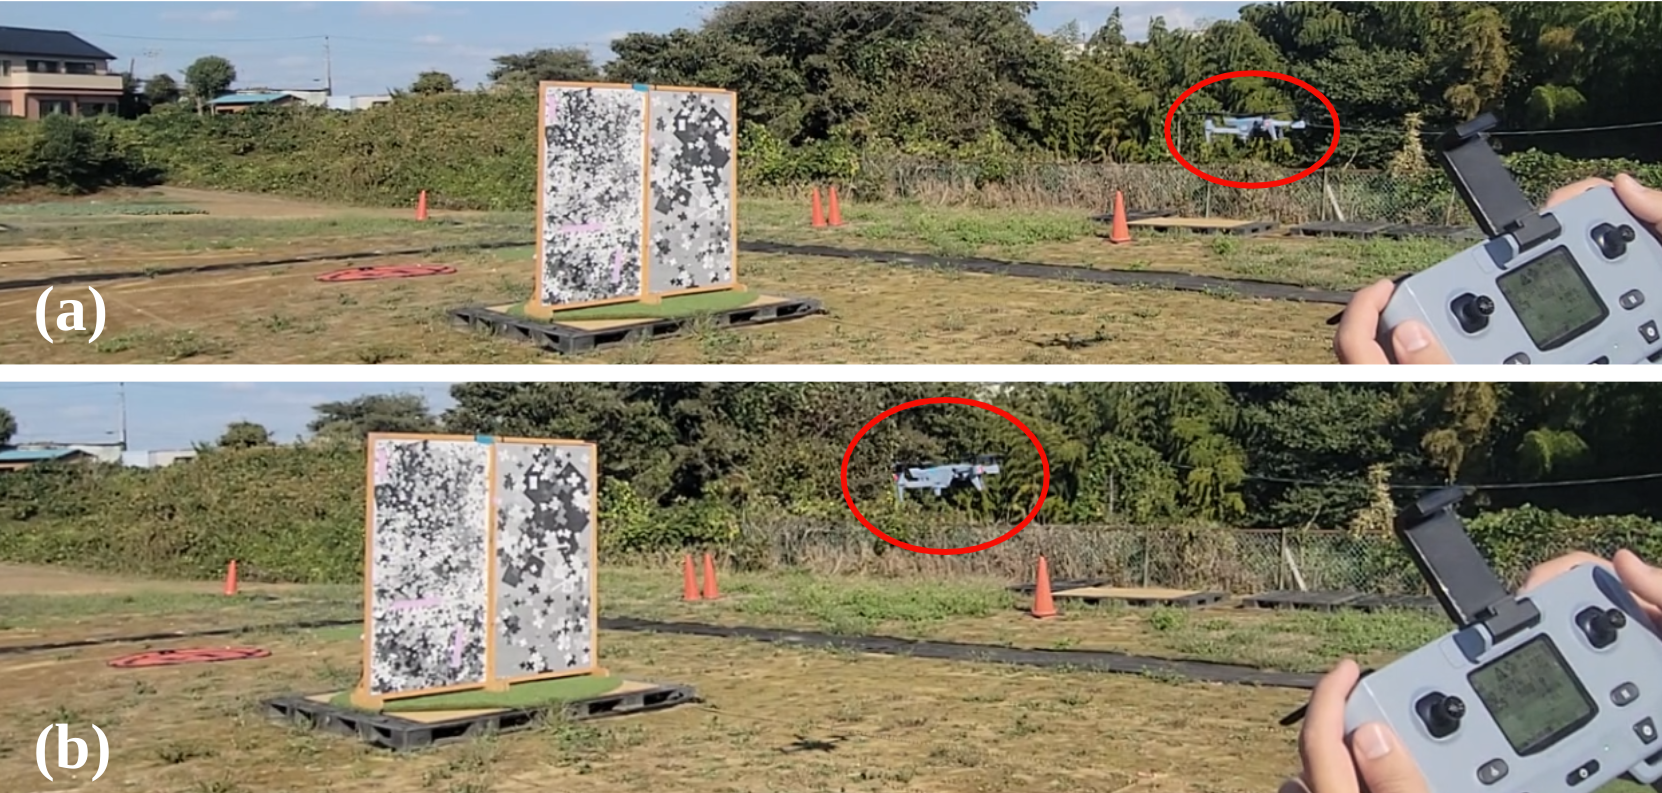
\includegraphics[scale=0.25]{partes/ImgJoao/real-1-single-3-frames-1.png}
    \caption[Capturas de una grabación de uno de los vuelos en entorno real con un obstáculo simple (1).]{Capturas de una grabación de uno de los vuelos en entorno real con un obstáculo simple (1). \textbf{(a)} Comienza el vuelo. \textbf{(b)} Se comienza a esquivar el obstáculo.}
    \label{real-1-single-3-frames-1}
\end{figure}

\begin{figure}[H]
    \centering
    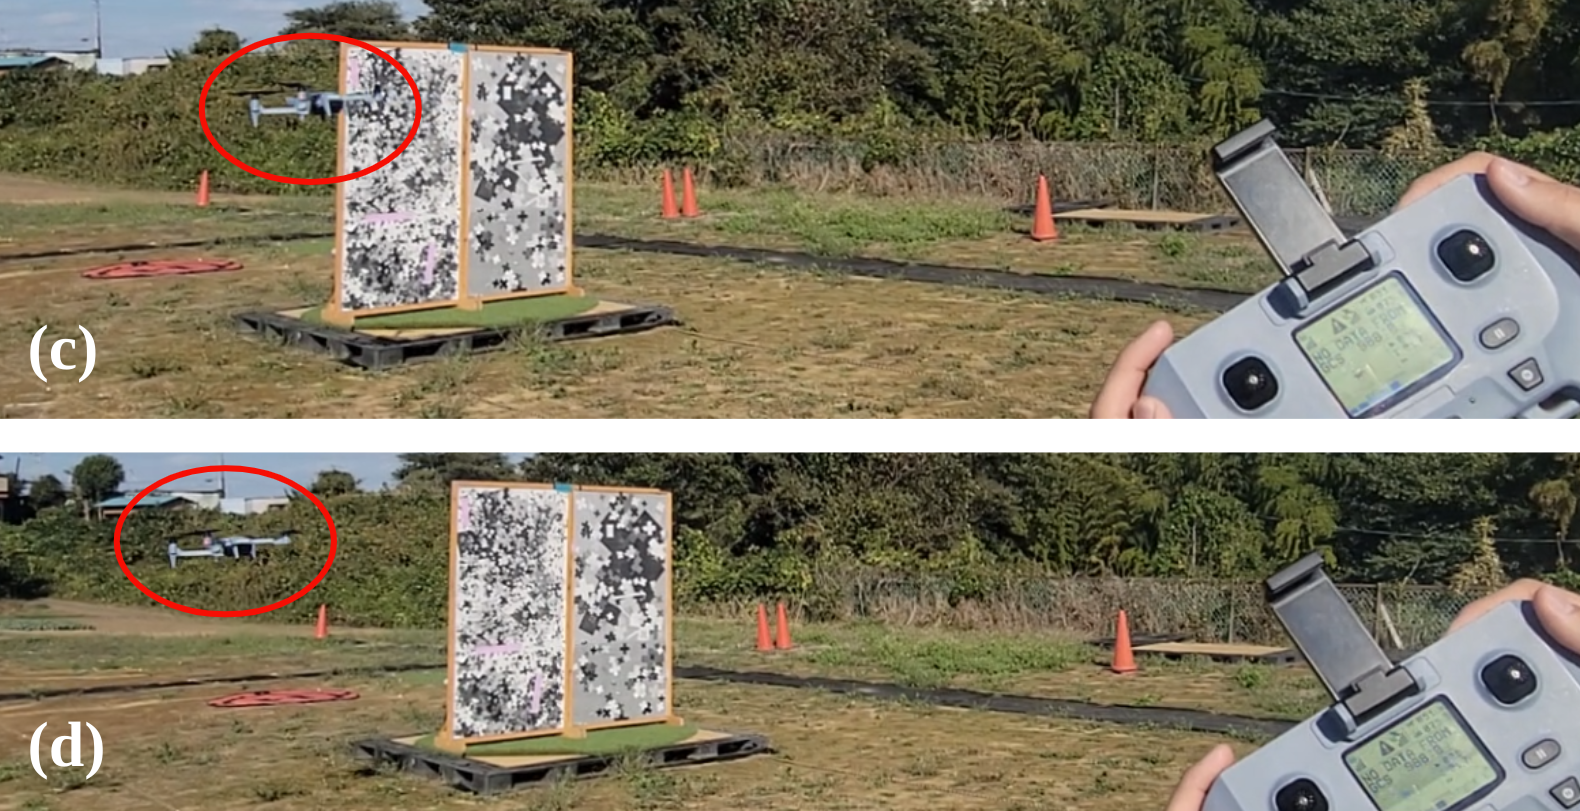
\includegraphics[scale=0.255]{partes/ImgJoao/real-1-single-3-frames-2.png}
    \caption[Capturas de una grabación de uno de los vuelos en entorno real con un obstáculo simple (2).]{Capturas de una grabación de uno de los vuelos en entorno real con un obstáculo simple (2). En \textbf{(c)} y \textbf{(d)}, se esquiva el obstáculo por el flanco izquierdo.}
    \label{real-1-single-3-frames-2}
\end{figure}

\begin{figure}[H]
    \centering
    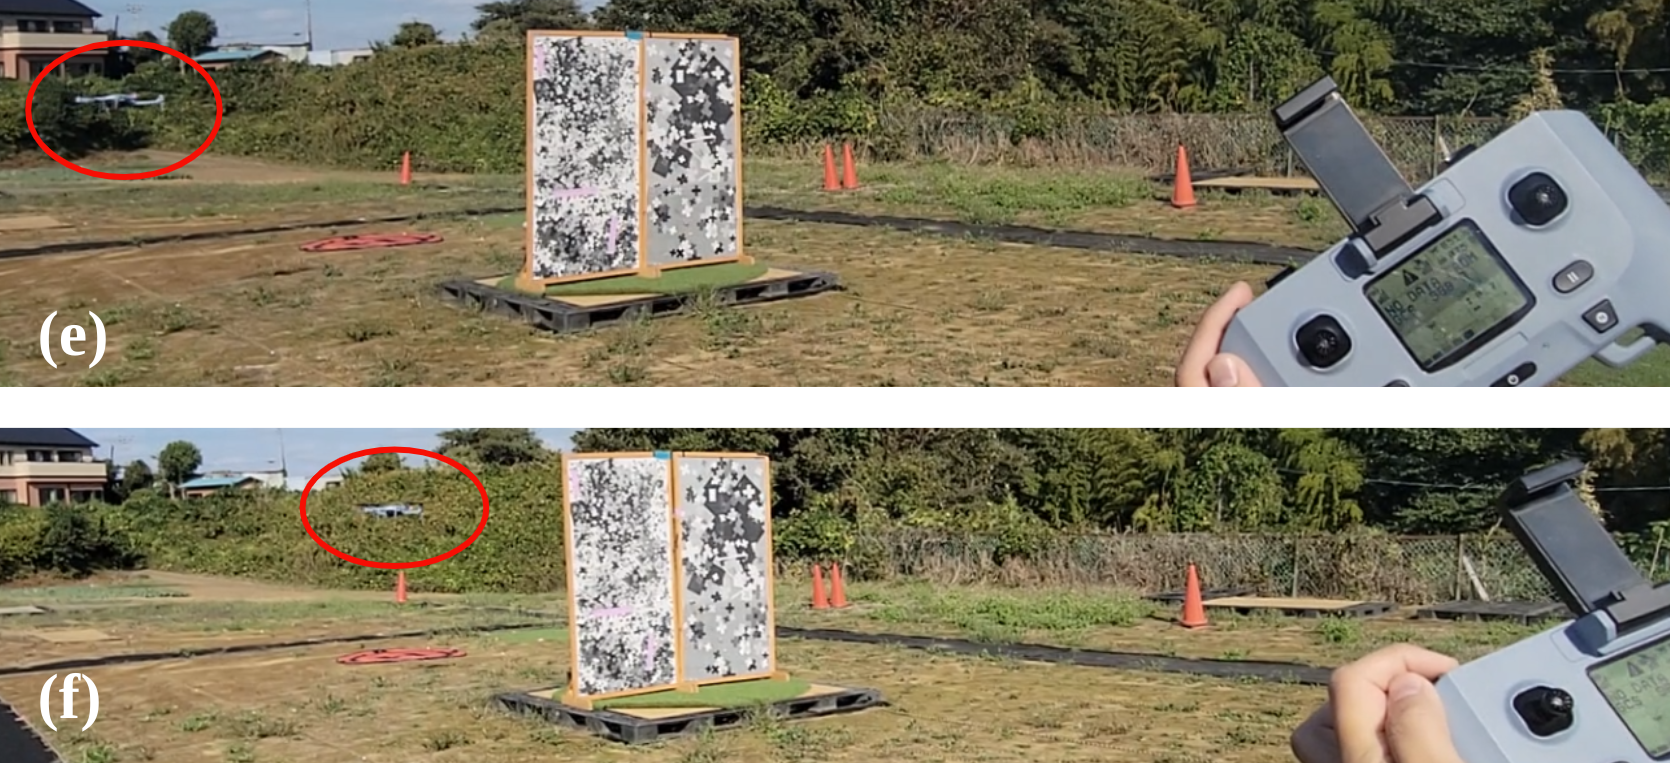
\includegraphics[scale=0.245]{partes/ImgJoao/real-1-single-3-frames-3.png}
    \caption[Capturas de una grabación de uno de los vuelos en entorno real con un obstáculo simple (3).]{Capturas de una grabación de uno de los vuelos en entorno real con un obstáculo simple (3). En \textbf{(e)} y \textbf{(f)}, como no se observan obstáculos, se navega en dirección a la meta.}
    \label{real-1-single-3-frames-3}
\end{figure}

\begin{figure}[H]
    \centering
    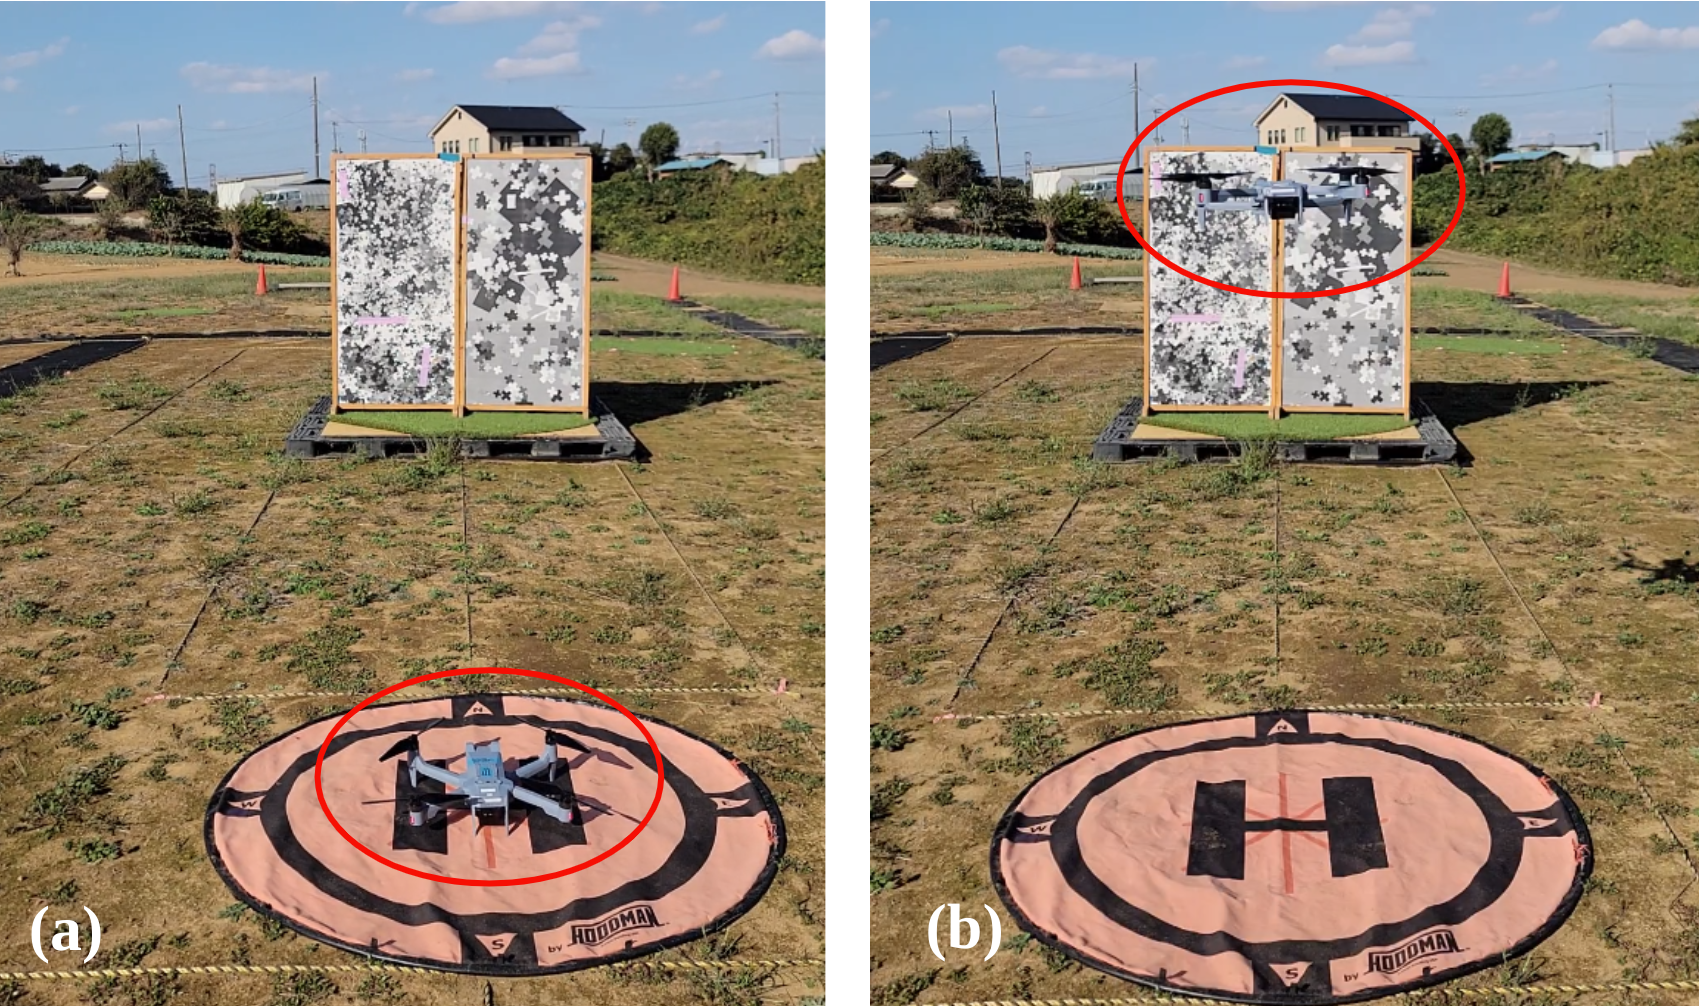
\includegraphics[scale=0.24]{partes/ImgJoao/real-1-single-4-frames-1.png}
    \caption[Capturas de una grabación de uno de los vuelos en entorno real con un obstáculo simple. Vista frontal (1).]{Capturas de una grabación de uno de los vuelos en entorno real con un obstáculo simple. Vista frontal (1). \textbf{(a)} Antes del despegue. \textbf{(b)} Comienza el vuelo.}
    \label{real-1-single-4-frames-1}
\end{figure}

\begin{figure}[H]
    \centering
    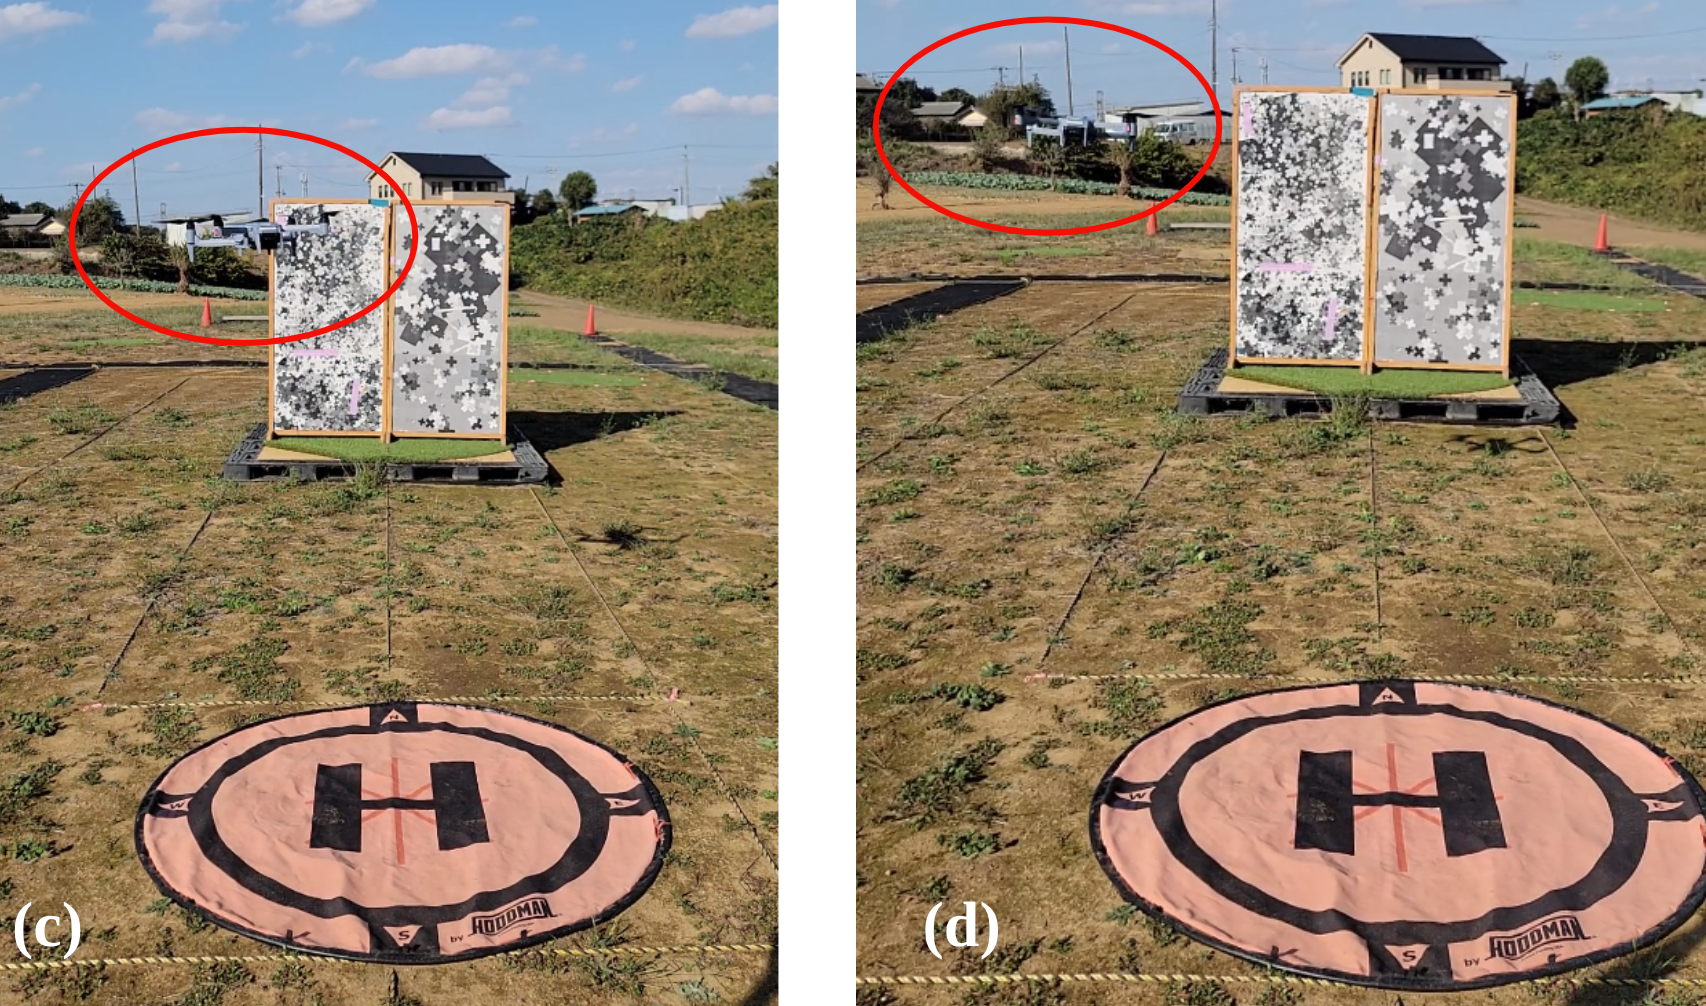
\includegraphics[scale=0.24]{partes/ImgJoao/real-1-single-4-frames-2.png}
    \caption[Capturas de una grabación de uno de los vuelos en entorno real con un obstáculo simple. Vista frontal (2).]{Capturas de una grabación de uno de los vuelos en entorno real con un obstáculo simple. Vista frontal (2). En \textbf{(c)} y \textbf{(d)}, se esquiva el obstáculo por el flanco izquierdo.}
    \label{real-1-single-4-frames-2}
\end{figure}

\begin{figure}[H]
    \centering
    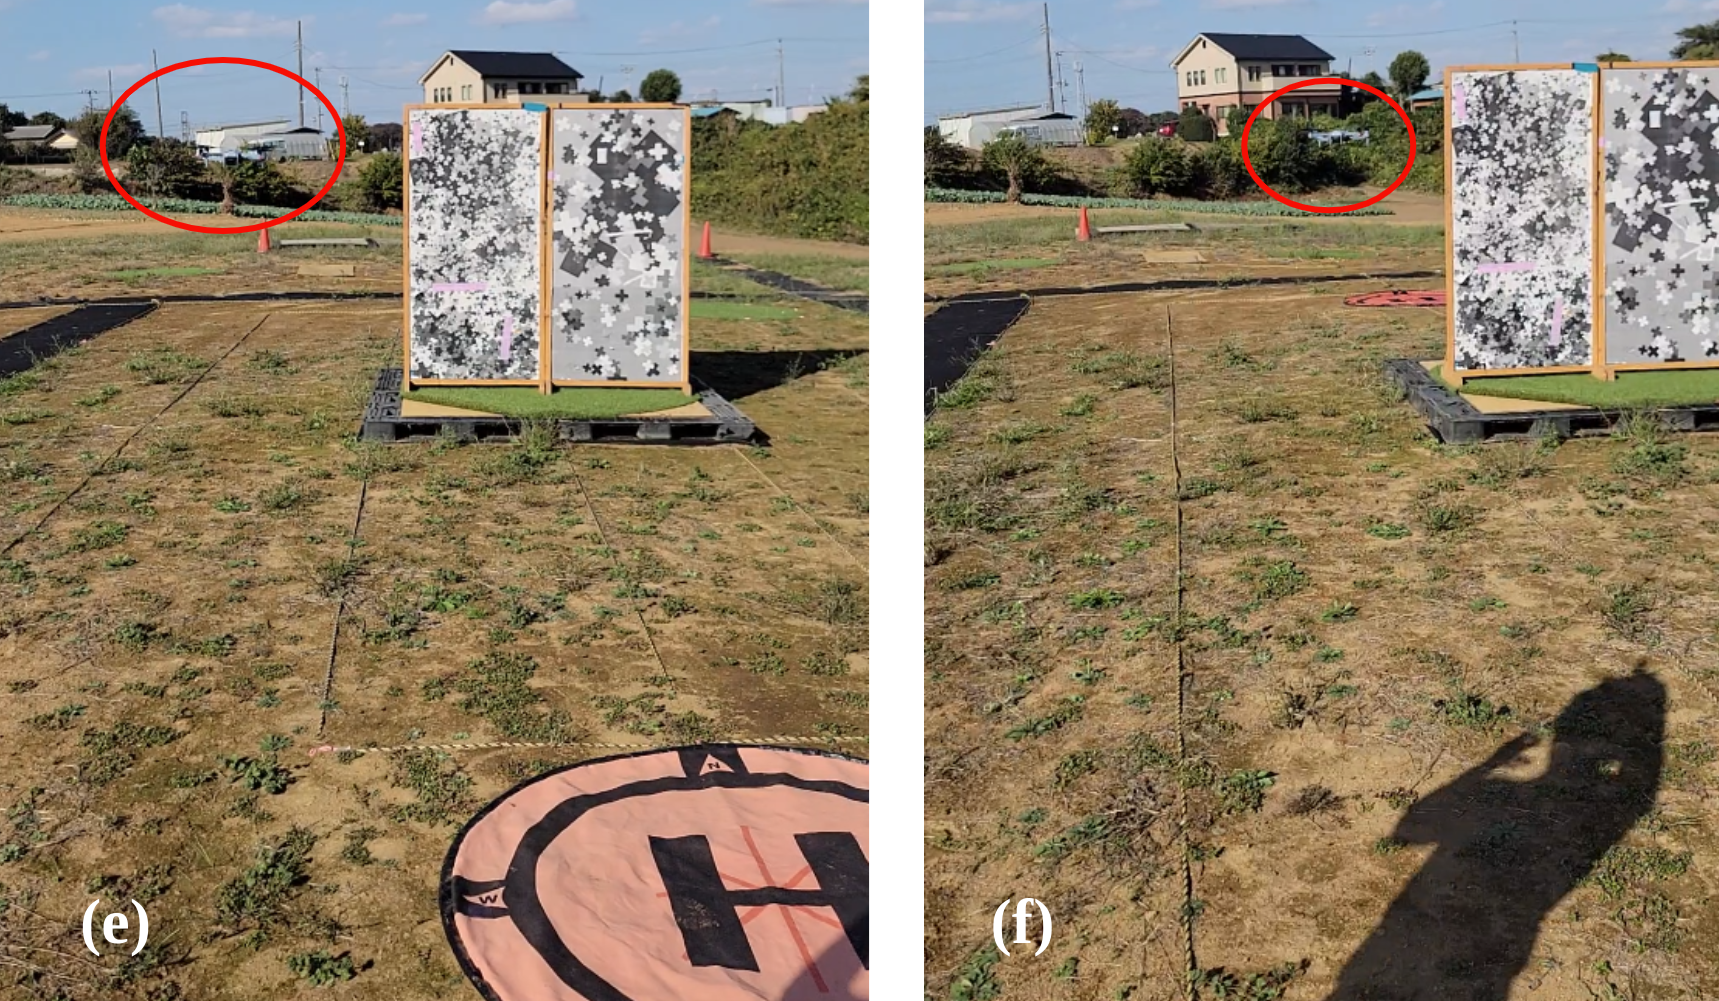
\includegraphics[scale=0.24]{partes/ImgJoao/real-1-single-4-frames-3.png}
    \caption[Capturas de una grabación de uno de los vuelos en entorno real con un obstáculo simple. Vista frontal (3).]{Capturas de una grabación de uno de los vuelos en entorno real con un obstáculo simple. Vista frontal (3). En \textbf{(e)} y \textbf{(f)}, como no se observan obstáculos, se navega en dirección a la meta.}
    \label{real-1-single-4-frames-3}
\end{figure}

La segunda configuración de obstáculos utilizada fue una configuración con dos obstáculos paralelos con una separación entre si, esta separación fue distinta para cada vuelo. A diferencia de la configuración anterior, en esta configuración solo se hicieron 3 vuelos. El objetivo de estos vuelos era observar el comportamiento del algoritmo en este escenario, en particular, confirmar la presencia de la tendencia certera de esquivar obstáculos por el flanco izquierdo que se observó durante vuelos análogos en entornos de simulación; así como también observar si esta tendencia produce colisiones inminentes.

En el primer vuelo en esta configuración se utilizó una separación de 3 metros, la figura \ref{real-2-parallelA-0-config} muestra una fotografía que ilustra la configuración utilizada. Este vuelo fue abortado por colisión inminente, la figura \ref{real-2-parallelA-1-frames} muestra capturas de la grabación de este vuelo en donde se observa el comportamiento del algoritmo. Primero (\ref{real-2-parallelA-1-frames}(a)), la ejecución comienza; segundo (\ref{real-2-parallelA-1-frames}(b)), el QUAV se dirige hacia el espacio entre ambos obstáculos en lugar de esquivar los obstáculos por el flanco derecho; y tercero (\ref{real-2-parallelA-1-frames}(c)), cuando el obstáculo derecho sale del campo de visión, el algoritmo intenta esquivar el obstáculo que aun es visible por el flanco izquierdo, lo cual produce una colisión inminente, haciendo que el piloto tenga que abortar el vuelo. Estos resultados coinciden con el comportamiento observado en simulación \footnote{Vea la figura \ref{fig:depth-parallel-5}}, y confirman la presencia de la tendencia certera a esquivar obstáculos por el flanco izquierdo.

\begin{figure}[H]
    \centering
    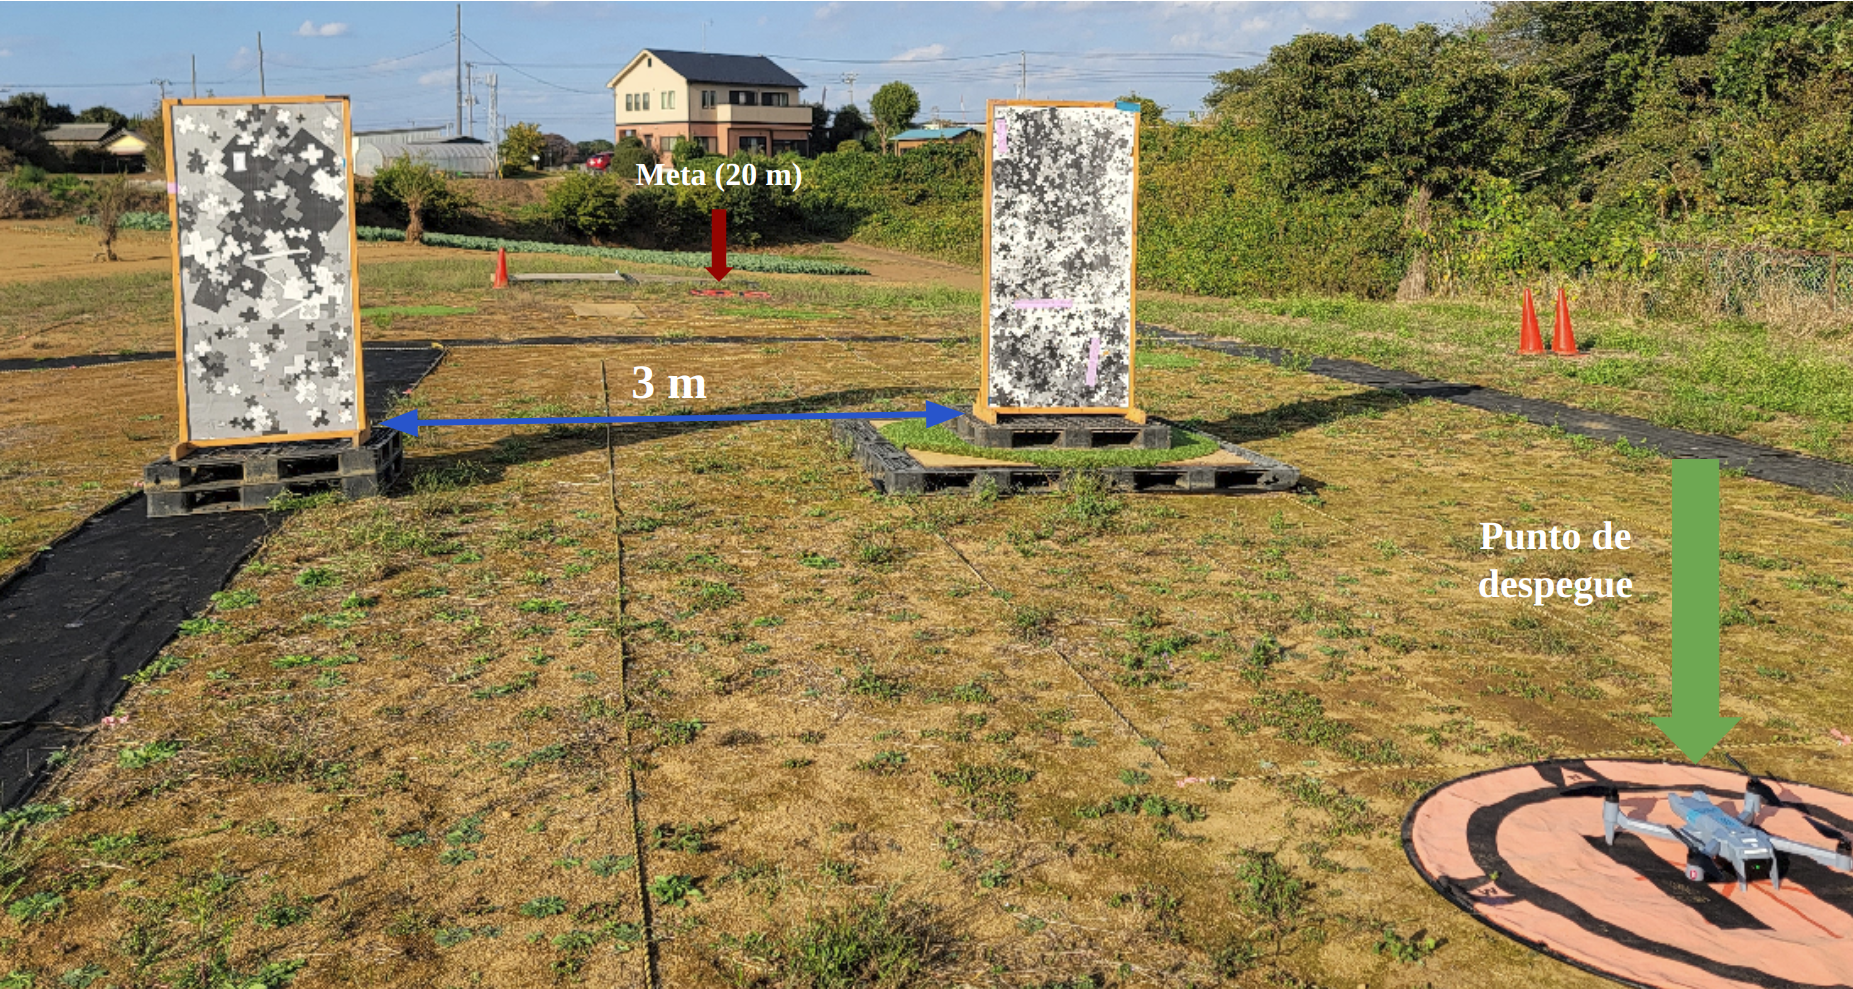
\includegraphics[scale=0.22]{partes/ImgJoao/real-2-parallelA-0-config.png}
    \caption[Configuración de obstáculos en entorno real: Obstáculos paralelos a 3 metros de separación.]{Configuración de obstáculos en entorno real: Obstáculos paralelos a 3 metros de separación.}
    \label{real-2-parallelA-0-config}
\end{figure}

\begin{figure}[H]
    \centering
    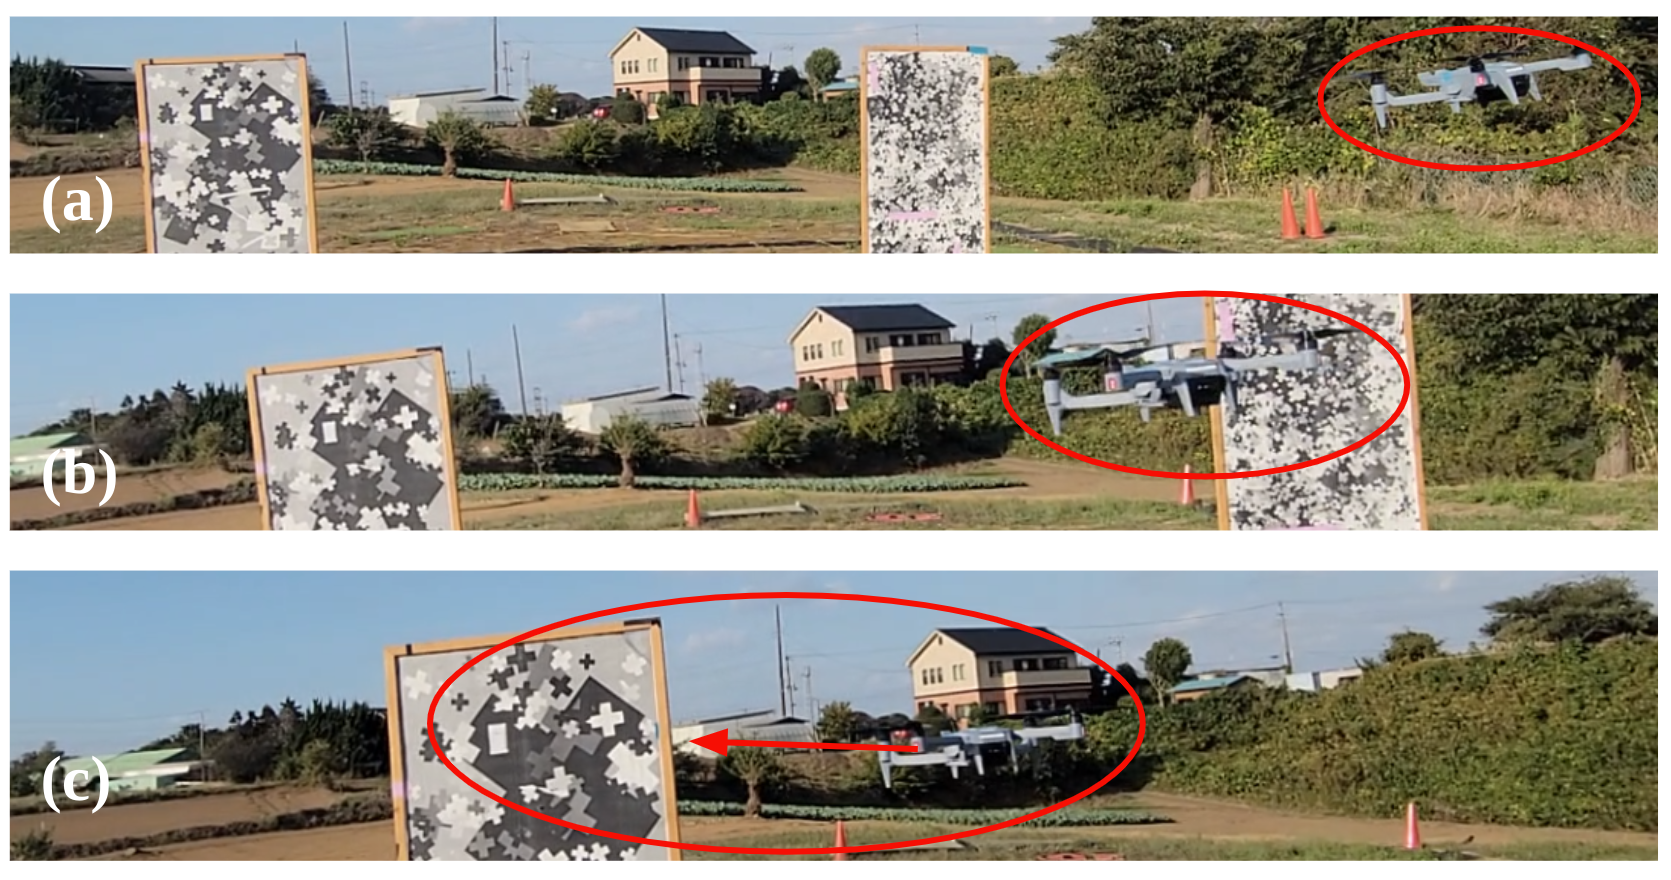
\includegraphics[scale=0.25]{partes/ImgJoao/real-2-parallelA-1-frames.png}
    \caption[Capturas de la grabación del vuelo en entorno real con obstáculos paralelos a 3 metros de separación.]{Capturas de la grabación del vuelo en entorno real con obstáculos paralelos a 3 metros de separación. \textbf{(a)} La ejecución comienza. \textbf{(b)} El QUAV se dirige hacia el espacio entre ambos obstáculos en lugar de esquivar los obstáculos por el flanco derecho. \textbf{(c)} Cuando el obstáculo derecho sale del campo de visión, el algoritmo intenta esquivar el obstáculo que aun es visible por el flanco izquierdo, lo cual produce una colisión inminente.}
    \label{real-2-parallelA-1-frames}
\end{figure}

El segundo vuelo en la configuración de obstáculos paralelos utilizó una separación de 4 metros, la figura \ref{real-3-parallelB-0-config} muestra una fotografía que ilustra la configuración utilizada. Este vuelo resultó exitoso, la figura \ref{real-3-parallelB-1-frames} muestra capturas de la grabación de este vuelo en donde se observa el comportamiento del algoritmo. Primero (\ref{real-3-parallelB-1-frames}(a)), la ejecución comienza y el QUAV navega hacia el espacio entre los dos obstáculos; segundo (\ref{real-3-parallelB-1-frames}(b)), esta vez, el obstáculo izquierdo sale del campo de visión, y el QUAV continúa hacia el espacio entre los dos obstáculos; y tercero (\ref{real-3-parallelB-1-frames}(c)), se superan los obstáculos y se navega en dirección a la meta. De este vuelo confirmamos que si la configuración de obstáculos paralelos es tal que el primer obstáculo que desaparece el campo de visión es el obstáculo izquierdo, entonces es posible que el algoritmo sea capaz de completar el vuelo sin producir colisiones.

\begin{figure}[H]
    \centering
    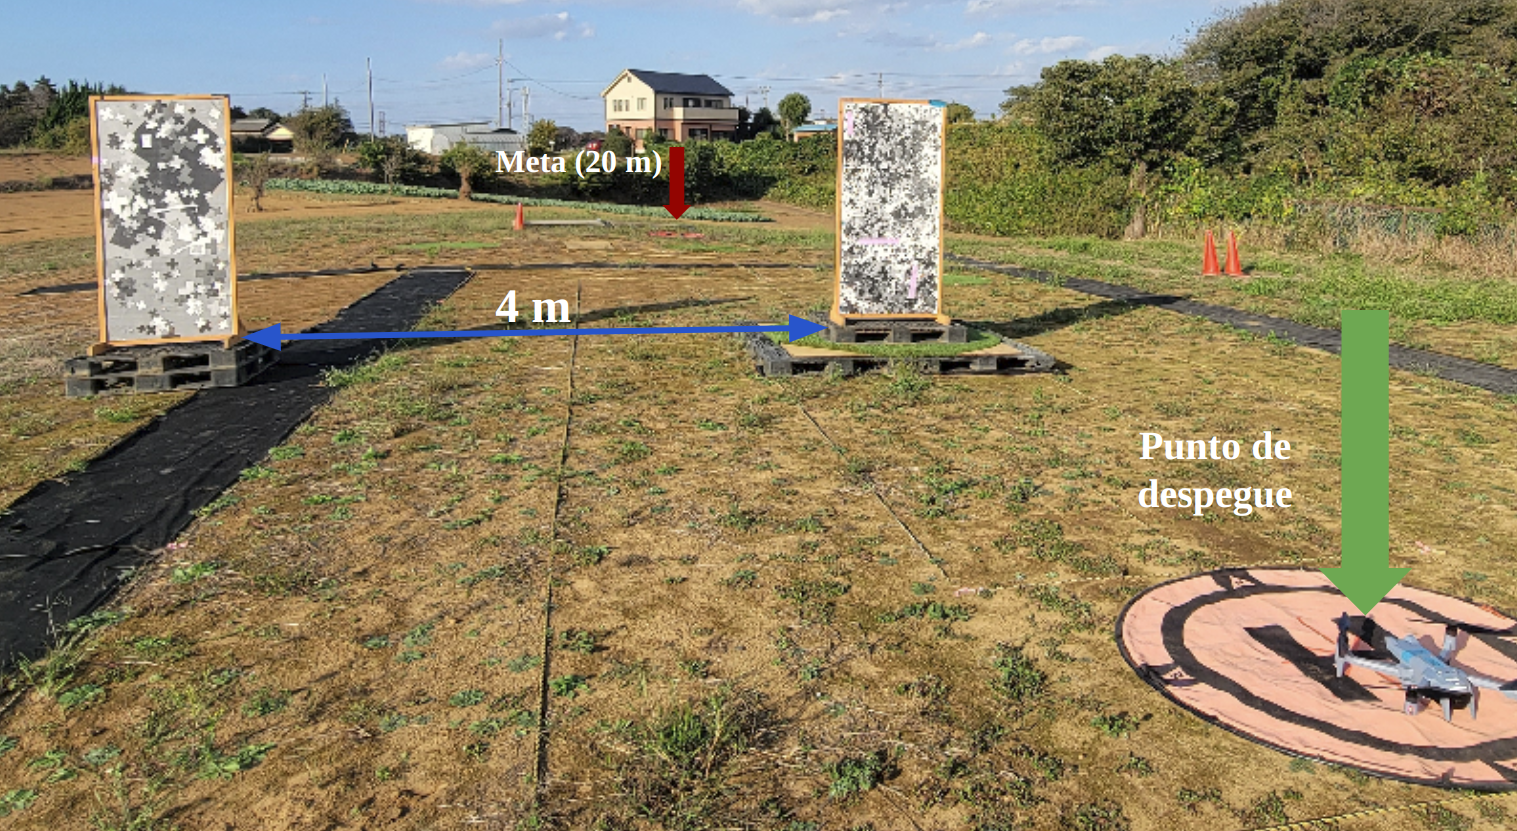
\includegraphics[scale=0.27]{partes/ImgJoao/real-3-parallelB-0-config.png}
    \caption[Configuración de obstáculos en entorno real: Obstáculos paralelos a 4 metros de separación.]{Configuración de obstáculos en entorno real: Obstáculos paralelos a 4 metros de separación.}
    \label{real-3-parallelB-0-config}
\end{figure}

\begin{figure}[H]
    \centering
    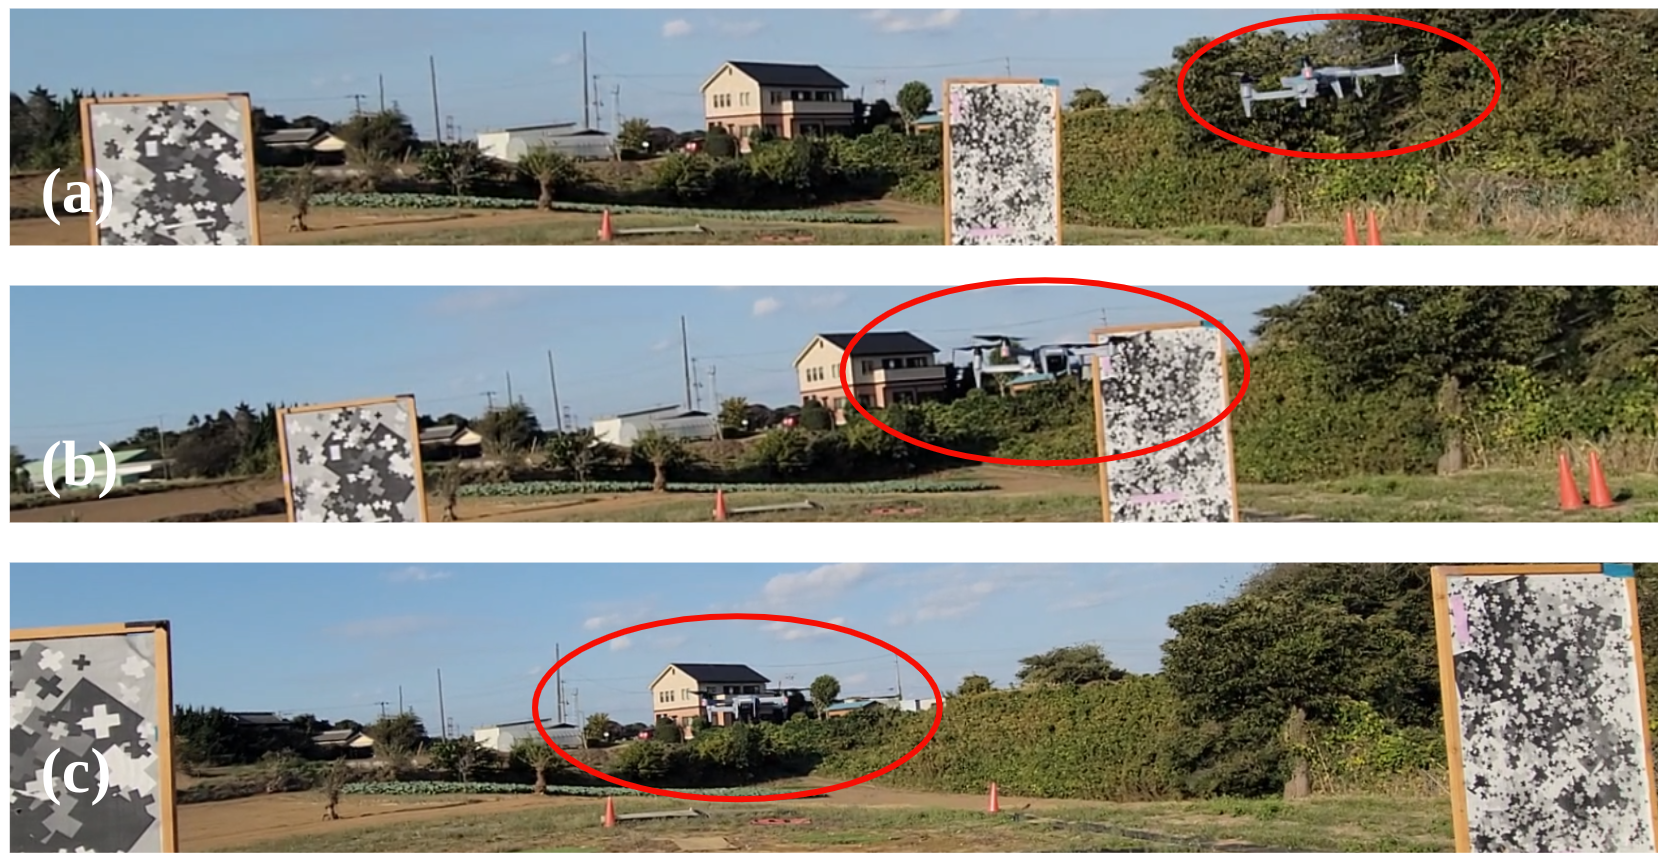
\includegraphics[scale=0.25]{partes/ImgJoao/real-3-parallelB-1-frames.png}
    \caption[Capturas de la grabación del vuelo en entorno real con obstáculos paralelos a 4 metros de separación.]{Capturas de la grabación del vuelo en entorno real con obstáculos paralelos a 4 metros de separación. \textbf{(a)} La ejecución comienza y el QUAV navega hacia el espacio entre los dos obstáculos. \textbf{(b)} El obstáculo izquierdo sale del campo de visión, y el QUAV continúa hacia el espacio entre los dos obstáculos. \textbf{(c)}  Se superan los obstáculos y se navega en dirección a la meta.}
    \label{real-3-parallelB-1-frames}
\end{figure}

El tercer y ultimo vuelo en la configuración de obstáculos paralelos utilizó una separación de 1 metro, la figura \ref{real-3-parallelB-0-config} muestra una fotografía que ilustra la configuración utilizada. Este vuelo resultó exitoso y la razón por la cual fue exitoso provee información adicional sobre la capacidad de evasión de obstáculos del algoritmo. La figura \ref{real-4-parallelC-1-frames} muestra capturas de la grabación de este vuelo en donde se observa el comportamiento del algoritmo. Primero (\ref{real-4-parallelC-1-frames}(a)), la ejecución comienza y el QUAV navega hacia el espacio entre los dos obstáculos; segundo, en el momento que el obstáculo izquierdo se vuelve el obstáculo mas grande en el campo de visión, el algoritmo intenta fuertemente corregir la trayectoria para esquivar el conjunto de obstáculos por el flanco izquierdo del obstáculo izquierdo, esto ocurre tempranamente en el vuelo pues la separación entre los obstáculos es relativamente pequeña; y tercero, como la decisión de de corregir la trayectoria hacia la izquierda ocurre de forma temprana, el algoritmo tiene tiempo de completar la trayectoria sin producir colisiones, resultando en una ejecución exitosa. El resultado de este vuelo expone que si existe el espacio y el tiempo para esquivar un conjunto de obstáculos por el flanco mas hacia la izquierda, es posible que la política de evasión de obstáculos sea capaz de completar el vuelo exitosamente.

\begin{figure}[H]
    \centering
    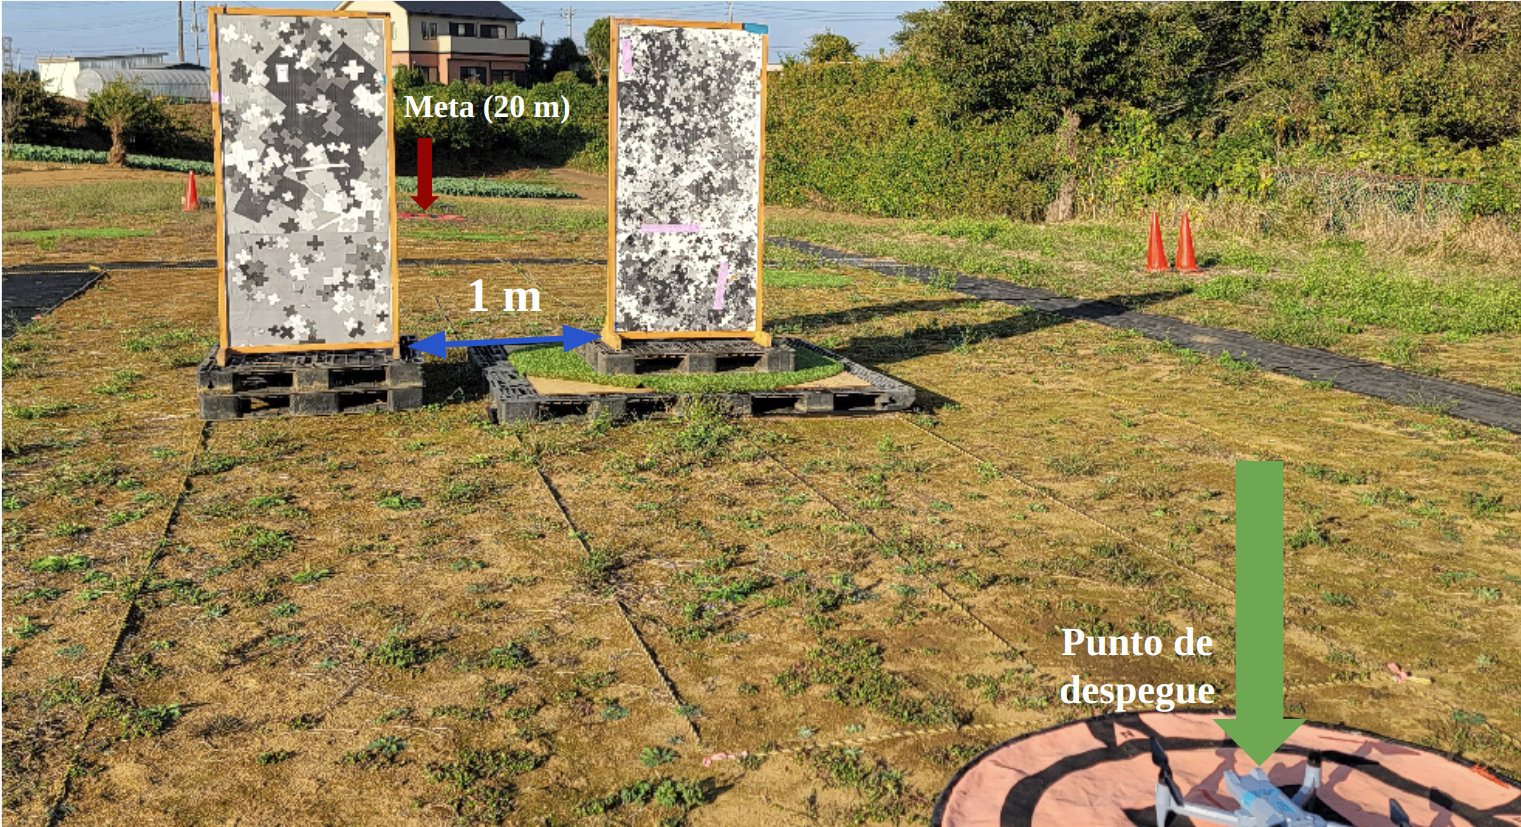
\includegraphics[scale=0.27]{partes/ImgJoao/real-4-parallelC-0-config.png}
    \caption[Configuración de obstáculos en entorno real: Obstáculos paralelos a 1 metro de separación.]{Configuración de obstáculos en entorno real: Obstáculos paralelos a 1 metro de separación.}
    \label{real-4-parallelC-0-config}
\end{figure}

\begin{figure}[H]
    \centering
    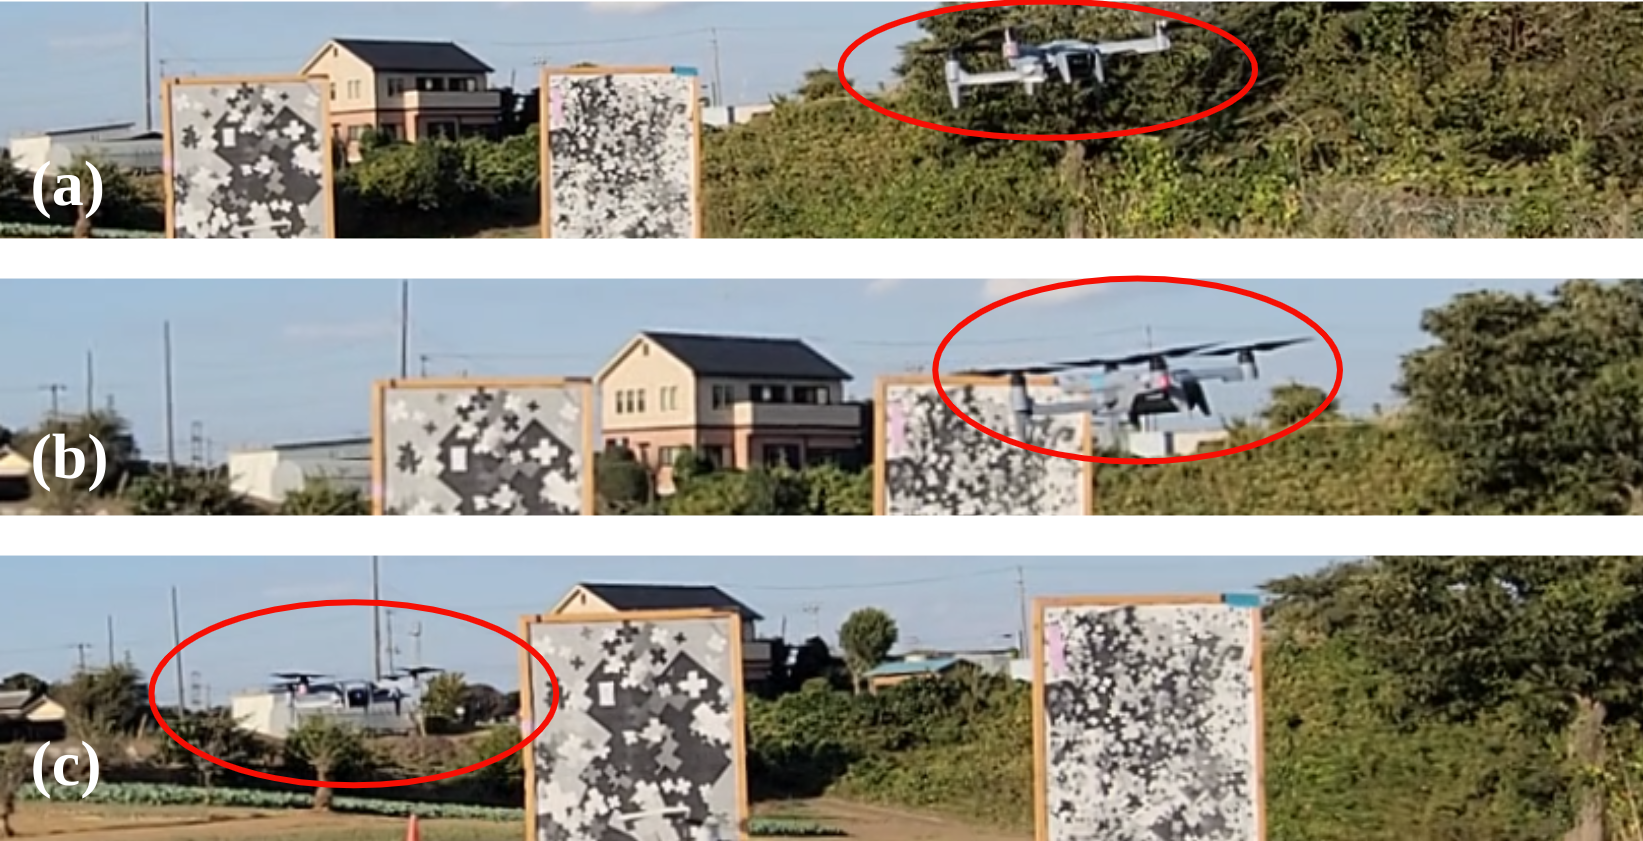
\includegraphics[scale=0.25]{partes/ImgJoao/real-4-parallelC-1-frames.png}
    \caption[Capturas de la grabación del vuelo en entorno real con obstáculos paralelos a 1 metro de separación.]{Capturas de la grabación del vuelo en entorno real con obstáculos paralelos a 1 metro de separación. \textbf{(a)} La ejecución comienza y el QUAV navega hacia el espacio entre los dos obstáculos. \textbf{(b)} El obstáculo izquierdo se vuelve el obstáculo mas grande en el campo de visión y el algoritmo intenta fuertemente corregir la trayectoria para esquivar el conjunto de obstáculos por el flanco izquierdo del obstáculo izquierdo. \textbf{(c)} Como la decisión de de corregir la trayectoria hacia la izquierda ocurre de forma temprana, el algoritmo tiene tiempo de completar la trayectoria sin producir colisiones, resultando en una ejecución exitosa. }
    \label{real-4-parallelC-1-frames}
\end{figure}

Los vuelos realizados permiten evaluar la estabilidad del algoritmo de evasión de obstáculos en entornos de la vida real, resaltando su consistencia, especialmente en la configuración de un obstáculo simple. No obstante, los resultados también revelan los efectos derivados de las dificultades encontradas durante el refinamiento fino de la política estudiante, manifestándose principalmente en la preferencia absoluta por esquivar obstáculos hacia el flanco izquierdo. Como consecuencia directa de estos vuelos, se exploran escenarios que ilustran el impacto de esta preferencia en situaciones de la vida real que involucran configuraciones de dos obstáculos paralelos. Dicho esto, finalmente, en la tabla \ref{table:real-results} se muestra un resumen de los resultados obtenidos en los vuelos en entornos de la vida real.

\begin{table}[h]
\centering
\begin{tabular}{||c || c | c | c||} 
 \hline
 \textbf{Configuración} & \jim{N_{total}} & \jim{N_{exito}} & \textbf{porcentaje de éxito} \\ [0.5ex] 
 \hline\hline
 Obstáculo simple              & 11 & 10 & 90\% \\ 
 \hline
 Dos obstáculos paralelos      & 3 &  2  & 66\% \\
 \hline
\end{tabular}
\caption[Resumen de los resultados obtenidos en los vuelos en entornos de la vida real.]{Resumen de los resultados obtenidos en los vuelos en entornos de la vida real. \jim{N_{total}} y \jim{N_{exito}} son el numero de vuelos totales y sin colisión inminente respectivamente.}
\label{table:real-results}
\end{table}

\section{Resumen}

Este capítulo abordó la evaluación y presentación de los resultados obtenidos, proporcionando una perspectiva crítica sobre el rendimiento de la solución propuesta. En la Sección \ref{sec:results-finetune}, se exploraron los resultados del ajuste fino de la política estudiante, destacando los desafíos asociados al sobre-ajuste de los datos de entrenamiento y a la generación de la base de datos. Además, se aclaró que, debido a limitaciones de tiempo de desarrollo y recomendaciones del equipo de ACSL, no se abordó completamente el problema del sobre-ajuste, lo que produjo efectos evidentes al evaluar la política de evasión de obstáculos. En particular, se observó cómo esta decisión ha llevado a una fuerte preferencia de la política por esquivar obstáculos por el flanco izquierdo.

La sección \ref{sec:results-flights} detalló los resultados de la política de evasión de obstáculos, presentando los vuelos en simulación en la subsección \ref{sec:results-AirSim} y los vuelos sobre la plataforma física de implementación, SOTEN, en la subsección \ref{sec:results-SOTEN}. Estos resultados ofrecieron una perspectiva del rendimiento de la solución en configuraciones simples de obstáculos, donde la política de evasión se mostró estable. También se exploraron configuraciones donde la fuerte preferencia de la política por esquivar obstáculos por el flanco izquierdo produjo colisiones, y se observaron distintos escenarios y consecuencias de ello.

En resumen, este capítulo proporcionó una evaluación que sirve de base para la discusión del siguiente capítulo, el de conclusiones. El contexto introducido en este capítulo también permite considerar direcciones para trabajos futuros que se construyan sobre la implementación presentada en este trabajo.
